\documentclass[english,a4paper,oneside]{amsart}

\newcommand{\scr}[1]{\mathscr{#1}}
\usepackage{hyperref}
%\usepackage{showkeys}
\usepackage{graphicx}
\usepackage{verbatim}
\usepackage{subcaption}


\hypersetup{
 hidelinks,colorlinks=false,breaklinks=true,
 pdfkeywords={machine learning, deep learning, transfer learning, collaborative learning, ResNet, convolutional neural networks},
 pdfauthor={Justin Noel},
}
\usepackage{Definitions}
\usepackage{Environments2}
\usepackage{PageSetup}
\usepackage{amssymb}
%\usepackage{draftwatermark} %For the watermark in the background
\usepackage{datetime} %To access the time of writing
%\SetWatermarkScale{1.85}
% \SetWatermarkAngle{58}
% \SetWatermarkLightness{0.85}
% \SetWatermarkText{\shortstack{Draft \vspace{4pc}\\\vspace{4pc}{\mmddyyyydate\today}\  \currenttime}}
\usepackage{enumitem} %Used for individualized enumerate labellings 
\usepackage{geometry} %allows customization of margins and changing paper sizes
\usepackage[toc,page]{appendix} %Adding appendix
\usepackage{mathtools} %left subscripts
% \usepackage[notref,notcite]{showkeys}

% The following adds todos and notes
\usepackage[
disable=true, % uncomment for disabling
color=orange!80, % default color
bordercolor=black,
textwidth=.8in,
textsize=small]
{todonotes}

\usepackage{caption} %Need for blank figure label
%This allows one to have subfigures next to each other
\usepackage{subcaption}
\DeclareCaptionSubType[Alph]{figure}
\captionsetup[subfigure]{labelformat=parens}

% \renewcommand\thesubfigure{(\Alph{subfigure})}
%Change math fonts

%Niko: The following doesn't compile on my portable so it's commented out at times.

\usepackage[bb=ams, cal=euler, scr=rsfso]{mathalfa}

\crefname{axiom}{Axiom}{Axioms}

%Better tables
\usepackage{tabu}
% the following is necessary for compatibility with amsart
\makeatletter \providecommand\@dotsep{5}
\makeatother
% for compatibility with amsart:
% use \amsartlistoftodos to make list of todos
\newcommand{\amsartlistoftodos}{\makeatother \listoftodos\relax}
%
% notes made by Akhil
\newcommand{\anote}[1]{\todo[inline,color=red!35]{#1}}
\newcommand{\ampar}[1]{\todo[color=red!35]{#1}}
\newcommand{\acom}[1]{\todo[noline,color=red!35]{#1}}

% notes made by Niko
\newcommand{\nnote}[1]{\todo[inline,color=blue!35]{#1}}
\newcommand{\nmpar}[1]{\todo[color=blue!35]{#1}}
\newcommand{\ncom}[1]{\todo[noline,color=blue!35]{#1}}
%
% notes made by Justin
\newcommand{\jnote}[1]{\todo[inline,color=green!40]{#1}}
\newcommand{\jmpar}[1]{\todo[color=green!35]{#1}}
\newcommand{\jcom}[1]{\todo[noline,color=green!35]{#1}}

% \newcommand{\lsub}[2]{\prescript{}{#1}{#2}}
\newcommand{\Desc}{\mathrm{Desc}}
\newcommand{\fun}{\mathrm{Fun}}
\newcommand{\Fun}{\mathrm{Fun}}
\newcommand{\ev}{\mathrm{ev}}
\newcommand{\md}{\mathrm{Mod}}
\newcommand{\NSpectra}{\category{NSpectra}}
\newcommand{\CoInd}{\mathrm{Coind}}
\newcommand{\Coind}{\mathrm{Coind}}
\newcommand{\Res}{\mathrm{Res}}
\renewcommand{\Top}{{\mathcal{S}}}
\newcommand{\psTop}{{\category{T}}}
\newcommand{\catS}{\category{S}}
\newcommand{\catC}{\category{C}}
\newcommand{\catD}{\category{D}}
\usepackage{url} %For writing our URL's
\renewcommand{\ho}{\mathrm{Ho}\,}
\newcommand{\Spec}{\mathrm{Spec}}
\newcommand{\SpG}{\mathrm{Sp}_G}
\newcommand{\SpH}{\mathrm{Sp}_H}
\newcommand{\SpK}{\mathrm{Sp}_K}
\newcommand{\Spe}{\mathrm{Sp}}
\theoremstyle{definition}
\newtheorem{thmA}{Theorem}

\renewcommand\thethmA{\Alph{thmA}}

\renewcommand\Im{\mathrm{Im}}
\Crefname{thmA}{Theorem}{Theorems}
\newcommand{\sOG}{\sO(G)}
\newcommand{\sOH}{\sO(H)}
\newcommand{\ZOG}{\bZ\sO(G)}
\newcommand{\ZOGF}{\bZ\sO(G)_{\sF}}
\newcommand{\ZOGC}{\bZ\sO(G)_{\sC}}
\newcommand{\AG}{\sA(G)}
\newcommand{\ZAG}{\bZ\sA(G)}
\newcommand{\sOGF}{\sO(G)_{\sF}}
\newcommand{\sOHF}{\sO(H)_{\sF\cap H}}
\newcommand{\sOGEp}{\sO(G)_{\sE_p}}
\newcommand{\sOGA}{\sO(G)_{\sA}}
\newcommand{\sOGC}{\sO(G)_{\sC}}
\newcommand{\sBG}{\sB(G)}
\newcommand{\bb}[1]{\underline{#1}}
\newcommand{\sAll}{\sA\ell\ell}
\newcommand{\sAb}{\sA}
\newcommand{\sAbone}{\sAb^1}
\newcommand{\sAbn}{\sAb^n}
\newcommand{\sAbp}{\sAb_{(p)}}
\newcommand{\sTriv}{\sT}
% \newcommand{\sE}{\mathscr{E}}
\newcommand{\Tow}{\mathrm{Tow}}
\newcommand{\Townil}{\Tow^{\textrm{nil}}}
\newcommand{\Towfast}{\Tow^{\textrm{fast}}}
\newcommand{\sENil}{\sE^{\textrm{Nil}}}
\newcommand{\sEp}{\sE_{(p)}}
\newcommand{\sAllNil}{\sAll^{\textrm{Nil}}}
\newcommand{\bbsAllNil}{\bb{\sAll}^{\textrm{Nil}}}
\newcommand{\bbsAllTNil}{{\bb{\sAll}[T^{-1}]}^{\textrm{Nil}}}
\newcommand{\bbsAllpNil}{\sAll_{(p)}^{\textrm{Nil}}}
\newcommand{\sAllp}{\sAll_{(p)}}
\newcommand{\sAllpNil}{\sAll_{(p)}^{\textrm{Nil}}}
\newcommand{\oversFNil}{\overline{\sF}^{\textrm{Nil}}}
\newcommand{\sEpNil}{\sEp^{\textrm{Nil}}}
\newcommand{\sFNilPr}{{\sF^{\textrm{Nil}}}^\prime}
\newcommand{\sFNilPrPr}{{\sF^{\textrm{Nil}}}^{\prime\prime}}
\newcommand{\sFNil}{\sF^{\textrm{Nil}}}
\newcommand{\bbsFNil}{\bb{sF}^{\textrm{Nil}}}
\newcommand{\sFpNil}{\sF_{(p)}^{\textrm{Nil}}}
\newcommand{\sPNil}{\sP^{\textrm{Nil}}}
\newcommand{\sFone}{\sF_1}
\newcommand{\sFoneNil}{\sF_1^{\textrm{Nil}}}
\newcommand{\sFtwo}{\sF_2}
\newcommand{\sFtwoNil}{\sF_2^{\textrm{Nil}}}
\newcommand{\sFonetwoNil}{(\sF_1\cup\sF_2)^{\textrm{Nil}}}
\newcommand{\sFonecaptwoNil}{(\sF_1\cap\sF_2)^{\textrm{Nil}}}
\newcommand{\sGNil}{\sG^{\textrm{Nil}}}
\newcommand{\sGpNil}{\sG_{(p)}^{\textrm{Nil}}}
\newcommand{\sCNil}{\sC^{\textrm{Nil}}}
\newcommand{\sCp}{\sC_{(p)}}
\newcommand{\sCpNil}{\sC_{(p)}^{\textrm{Nil}}}
\newcommand{\sAbNil}{\sAb^{\textrm{Nil}}}
\newcommand{\sAbpNil}{\sAb_{(p)}^{\textrm{Nil}}}
\newcommand{\sAbpn}{\sAb_{(p)}^n}
\newcommand{\sAbpnNil}{\sA_{(p)}^{n,\textrm{Nil}}}
\newcommand{\GSpec}{\mathrm{Sp}_G}
\newcommand{\HSpec}{\mathrm{Sp}_H}
\newcommand{\KG}{KU}
\newcommand{\koG}{ko}
\newcommand{\KOG}{\mathit{KO}}
\newcommand{\kG}{ku}
\newcommand{\MUG}{\mathit{MU}}
\newcommand{\MOG}{\mathit{MO}}
\newcommand{\MUR}{M\bR}
\newcommand{\e}[1]{\mathbb{E}_{#1}}
\newcommand{\mdw}{\mathrm{Mod}^\omega}
\newcommand{\ko}{\bb{\mathit{ko}}}
\newcommand{\ku}{\bb{\mathit{ku}}}
\newcommand{\KO}{\bb{\mathit{KO}}}
\newcommand{\KU}{\bb{\mathit{KU}}}
\newcommand{\tmf}{\bb{\mathit{tmf}}}
\newcommand{\Tmf}{\bb{\mathit{Tmf}}}
\newcommand{\TMF}{\bb{\mathit{TMF}}}
\newcommand{\MO}{\bb{\mathit{MO}}}
\newcommand{\MSO}{\bb{\mathit{MSO}}}
\newcommand{\MSpin}{\bb{\mathit{MSpin}}}
%These two aren't underlined because they need to be localized first
\newcommand{\MString}{\mathit{MString}}
\newcommand{\MSp}{\mathit{MSp}}

\newcommand{\MSU}{\bb{\mathit{MSU}}}
\newcommand{\MUSix}{\bb{\mathit{MU}\langle 6\rangle}}
\newcommand{\Kn}{\bb{K(n)}}
\newcommand{\Gpi}{\pi_*^{(-)}}
\newcommand{\Gpit}{\pi_t^{(-)}}
\renewcommand{\mod}{\mathrm{Mod}}
\newcommand{\ring}{\mathrm{Ring}}
\renewcommand{\theenumi}{\arabic{enumi}}
\renewcommand{\labelenumi}{(\theenumi)}
\renewcommand{\theenumii}{\theenumi.{\arabic{enumii}}}
\renewcommand{\labelenumii}{(\theenumii)}
\makeatletter
\renewcommand{\p@enumii}{\theenumi.}
\makeatother
\setcounter{tocdepth}{2}

\newtheorem{cons}[thm]{Construction}
\begin{document}
	\title{A collaborative approach to deep learning}

	\author{Justin Noel}
	\address{University of Regensburg\\
	NWF I - Mathematik; Regensburg, Germany}
	\email{justin.noel@mathematik.uni-regensburg.de}
	\urladdr{http://nullplug.org}
	 \thanks{The author was partially supported by the DFG grants: NO 1175/1-1 and SFB 1085 - Higher Invariants, Regensburg. }


\date{\today}

\begin{abstract}
	We introduce several techniques for training collaborative ensembles of deep neural networks. In addition to learning to solve an image classification problem, these collaborative ensembles also learn to reach a consensus on their predictions. As a consequence, each of the models in these ensembles learns to mimic a traditional ensemble, with corresponding improvements to performance. %
\end{abstract}

\maketitle
 
\tableofcontents

\section{Definition}
\subsection{Project overview}
% Has an overview of the project been provided, such as the problem domain, project origin, and related datasets or input data? 
% Has enough background information been given so that an uninformed reader would understand the problem domain and following problem statement?
Recent advances in image classification have focused on constructing very deep and wide networks with 100+ layers \cite{ResNet,Inception}. While these networks represent the state of the art on standard benchmarks, training very deep and wide networks is extremely intensive computationally and introduces significant challenges to learning, typically due to vanishing gradients. Moreover, such models are often too slow at inference to be transferred to devices with limited computational resources, such as mobile devices. 

Shallow and thin networks are much faster to train and to perform inference with, but typically learn models which generalize relatively poorly to testing data. Research has shown that for shallow and wide networks, this is not so much an artifact of the shallow model's inability to express the deeper model's predictions \cite{Distillation,Shallow,Compression}, but rather, at least in part, the shallow model's tendency to overfit to the training data when given hard prediction targets. 

On the other side, it has been shown that training medium depth networks can be made easier by providing easier to match targets \cite{Curriculum, FitNet}.

% In this project we will consider a collaborative form of training deep networks for image classification problems on publicly available datasets.

\section{Problem Statement}

% Is the problem statement clearly defined? Will the reader understand what you are expecting to solve?
% Have you thoroughly discussed how you will attempt to solve the problem?
% Is an anticipated solution clearly defined? Will the reader understand what results you are looking for?

In this project we will investigate whether a \emph{collaborative} approach to learning can improve on the above state of affairs. To do this, we will train various models to solve an image classification problem using a variety of cost functions which will lead the models to reach a consensus on their outputs. By pushing the models to reach a consensus, we will show that each of the individual models will be able to better approximate the performance of the ensemble. 

A traditional ensemble typically outperforms each of its constituent models. Below we will see that collaboratively trained models learn to approximate the entire ensemble and outperform their corresponding models trained in isolation. The resulting collaborative ensembles have improved constituents and often improved ensemble performance. Since collaborative training is done concurrently with standard training, this improvement in performance comes at virtually no additional computational cost. %Since bagged ensembles typically have reduced generalization error, this would provide a new technique for improving the behavior of individual models, while removing the computational cost of running an ensemble. 

Below we will measure the generalization error in the usual fashion, via a test dataset and compare it to the outputs of models trained in the conventional, non-collaborative fashion. After examining the performance of a wide variety of collaboration methods. We will evaluate the training behavior by graphing the training and test errors of the best performing model.

More specifically, we will train two variations on the ResNet architecture \cite{ResNet}. Although we will leave the specifics of the implementation details to \cite{ResNet}, we will mention a few key properties. The general ResNet architecture can be easily scaled to varying depths by adjusting two parameters, the number of `bricks' $B$ and the number of repetitions $R$. With the exception of the last brick, each brick ends in a halving of each spatial dimension and a doubling of the number of filters. We adjust the width of the network by setting the number of filters $F$ for the first convolutional layer. All models are `fully convolutional' in the sense that they do not have any hidden fully connected layers. The resulting model will have $1+(B-1)(2R+2)+2R+1$ convolutational layers and end with a global average pooling operation and a linear map $\mathbb{R}^{2^B F} \to \mathbb{R}^{10}$ which is then composed with a softmax transformation. 

The first model will be a 'shallow and thin' model (ST) with $B=3, R=1$ and $F=8$, yielding a 10 layer model whose penultimate layer has dimension $2^{6}=64$.  This model has approximately 50k learnable parameters. The second model will be a `medium' (M) model with $B=3, R=2$, and $F=16$, yielding a 16 layer model whose penultimate layer has dimension $2^{7}=128$. This model has approximately 280k learnable parameters.  

Traditionally one might train these models simultaneously to form an ensemble and average their predictions in a suitable fashion. We can train both models simultaneously by applying gradient descent to minimize the sum of the two cost functions for the two models:
\begin{equation}\label{eq:ensemble}
 \mathrm{Cost^{ens}} = \mathrm{Cost}^{ST} + \mathrm{Cost}^{M}.
 \end{equation}
Typically, averaging the predictions reduces variance in the ensemble model's predictions and can improve generalization error. 

Below we will compare this approach to a collaborative approach, where after every iteration of training the models to the labeled data we will have the model `collaborate' by replacing \eqref{eq:ensemble} with 
\begin{equation}\label{eq:collab}
 \mathrm{Cost^{coll}} = \mathrm{Cost^{ens}} + \alpha \cdot \mathrm{Collab}.
\end{equation} 
Here $\mathrm{Collab}$ will be the `collaboration method' which will be one of three functions which measures the distance between the predictions produced by the models and $\alpha$ will be a `collaboration weight' which will dictate how much we want to emphasize collaboration versus learning from the hard targets. Both the choice of the collaboration method and the collaboration weight are hyperparameters. After this rephrasing, we can regard this project as a simple hyperparamter search.

\subsubsection{Collaborative learning}\label{sec:collab}
Before we make precise how our models will collaborate, we will recall how a neural network classifier is trained. Suppose that our classification problem is to find a function $f(x)=(f_1(x),\dots, f_n(x))$ approximating the labeling $x \mapsto y(x)=(y_1(x),\dots, y_n(x))$, here $y(x)$ is the one-hot encoding of a given classification of $x$ into one of $n$-classes. In other words, if $x$ belongs to the $i$th class, then $y_j(x)=\delta_{i,j}$. 

Our models will have the form \[f(x)=\textrm{Softmax}(g(x))=\frac{1}{\sum e^{g_i(x)}}(g_1(x),\dots, g_n(x)),\] where $g(x)$ is the vector of unscaled logits our model produces and implicitly a function of a parameter vector $\theta$. Such models are typically trained by attempting to minimize the cross-entropy of $f$ with $y(x)$:
\begin{align*}
CE(y(x), f(x)) &= - \sum y_j(x) \ln f_j(x)\\
&=-\ln f_i(x)\\
&=\ln(\sum e^{g_j(x)})-g_i(x).
\end{align*} 
Under this rephrasing we are trying to learn a function $g$ into $\mathbb{R}^n$ whose value will be as close to $+\infty$ as possible in the component corresponding to the positive classification and as close to $-\infty$ in each of the negative classification components. 

Since neural networks are trained by variants of gradient descent it can be helpful to calculate the gradient flow of the cross entropy function with respect to a parameter $\theta_k$:
\begin{align*}
 \frac{\partial CE(y(x), f(x))}{\partial \theta_k} &= \sum_\ell \frac{\partial CE(y(x), f(x))}{\partial g_\ell(x)} \frac{\partial g_\ell(x)}{\partial \theta_k} \\
 &=\sum_\ell \frac{e^{g_\ell(x)} \frac{\partial g_\ell(x)}{\partial \theta_k}}{\sum e^{g_m(x)}}-\delta_{\ell, i} \frac{\partial g_\ell(x)}{\partial \theta_k} \\
 &= \sum_\ell \frac{\partial g_\ell(x)}{\partial \theta_k}(f_\ell(x)-\delta_{\ell, i}).
 \end{align*}
 In particular, we used that $\frac{\partial CE(y(x), f(x))}{\partial g_\ell(x)}=f_\ell(x)-\delta_{\ell, i}.$ This means that the adjustment made to the $\ell$th unscaled logit to minimize the cross-entropy is proportional to the error in the $\ell$th prediction. 

 Note that the algorithm punishes all errors equally. For example, if the model produces the same value $g(x_1)=g(x_2)$ for two different training samples which should be labeled as class `7', then gradient descent will attempt to adjust the value of $g$ in the same way in each component for each sample. However, if $x_1$ `really looks like' a `1' and $x_2$ is definitively a `7' then perhaps it would make sense to not try to adjust the first component of $g(x_1)$ as much as the second component; doing so may make it harder for the model to classify ones correctly (see \Cref{Fig:Similar}). 

To understand this problem, so that we can solve it, consider the hypothesis that all possible inputs from our classification problem are pulled from some input space $M$ (which would be a manifold according to the manifold hypothesis). Our model is attempting to learn how to label the connected components of our manifold according to some omniscient labeling scheme $y$. It will do this by finding a projection $M\to \mathbb{R}^n$ which in the $i$th coordinate has only the image of the  $i$th labeled component of $M$ landing in the positive numbers. Over time the model pushes the values to greater and greater extremes and thus separates $M$ into components that are farther and farther away. 

The problem with this approach is that it actually assumes the components of $M$ are separable to begin with. In reality, it is not hard to image a sequence of seven's that gradually look more and more like a one (see \Cref{Fig:Similar}). If we take two arbitrarily close examples in $M$ which are assigned different classifications by $y$ the model learns to push these examples infinitely far from each other as fast as possible. A better approximation for our labeling problem should be fuzzier, where we assign to each point the degree the model should believe (in the Bayesian sense) a point lies in one class. This poses an easier task for optimization since not all classes need to be pushed so far apart and the model does not need to learn such a complicated embedding in order to separate them. 

Now the problem is to find appropriate soft targets for optimization. As such targets are not given to us, we can regard this as an unsupervised learning problem. A solution to this unsupervised learning problem is approximated by the solution to the supervised classification problem: As the model learns to classify the images, it produces soft targets that reflect the similarities between different images that the labels do not. 

So one can take two models, one which produces soft targets and another which trains to those soft targets. When this has been considered previously, this was done in two steps: first a very advanced model produces soft targets for a less complex model, which is then trained with these new target with the outcome that the less complex model outperforms the one trained on the hard targets (but still worse than the more advanced model).  This produces a model which is much faster at inference than the more advanced model, but with slightly degraded performance. 

We propose a similar implementation, but now we have the models learn simultaneously from each other. The models will partially target the hard targets, but the models will also learn to come to a consensus and produce approximately the same outputs.  This will be implemented by changing the cost function as in \eqref{eq:collab} by setting $\mathrm{Cost^{coll}}$ to be one of the following, where $f^{(1)}(x), f^{(2)}(x)$ are the prediction functions for the two models and $g^{(1)}(x), g^{(2)}(x)$ are their respective unscaled logits:
\begin{enumerate}
	\item (Symmetric cross entropy) \[\mathrm{Cost}^{CE}=-\left(\sum f^{(1)}_i(x)\ln f^{(2)}_i(x)+f^{(1)}_i(x)\ln f^{(1)}_i(x)\right).\]
	\item (L2-squared) $\mathrm{Cost}^{L2}=\sum (g_i^{(1)}(x)-g_i^{(2)}(x))^2$
	\item (L1) $\mathrm{Cost}^{L1}=\sum |g_i^{(1)}(x)-g_i^{(2)}(x)|.$
\end{enumerate}

All of these cost functions are clearly non-negative. The first two obviously have global minima when the two models produce identical unscaled logits, so the cost functions are zero. Turning to the symmetric cross entropy function, when the two models produce identical predictions then the symmetric cross entropy is equal to double the entropy of the (common) model's predicted distribution. If these models were able to minimizing the given cost function, then this distribution will have zero entropy and the model will have a global minimum. The upshot is that the collaborative models have theoretical global minima equal to those of their  non-collaborative models and, a priori, collaboration does not necessarily obstruct learning the ideal function.

On the other hand, it is clear that when $\alpha \gg 0$ is very large, the backpropagation algorithm will prioritize minimizing the collaboration cost function over the ensemble cost function. This forces to push the individual models to try to solve the classification problem \emph{while} producing identical predictions; a significantly more difficult task.

The hope is that we can train a simpler model to have much better performance characteristics than it would otherwise and perhaps better than that of a model constructed by distillation/compression techniques \cite{Distillation,Compression}, although we will not be able to test this hypothesis due to time and resource constraints (see \Cref{ouraxiom} below). 
% with respect to the hard targets to a linear combination of that cost function with either 1) the cross-entropy with the other model or 2) the average sum of squares difference between the unscaled logits of the two models.  The exact choice of cost function will be a hyperparameter that we will investigate. We note, by calculating the gradients, that choice 1) will cause the model outputs to converge uniformly toward each other, while 2) will cause the outputs to converge toward each other at a rate proportional to their difference. The second choice will have the outcome that it will force the models to be very close to each other rather quickly, while allowing the models to have a small amount of wiggle room when their outputs are on average less than a unit apart. 

\subsection{Metrics}
Below we will evaluate the models by examining the average value of their respective error and cost functions on the training and test sets over the course of the training period.  We will show that the test error rate for the ST and M models will nearly always be lower than those of the models trained in a traditional ensemble. %We hope that the M model will learn faster in the collaborative fashion and we should be able to witness this by examining the value of the training costs over the course of the training. 

\section{Analysis}
% If a dataset is present for this problem, have you thoroughly discussed certain features about the dataset? Has a data sample been provided to the reader?
% If a dataset is present for this problem, are statistics about the dataset calculated and reported? Have any relevant results from this calculation been discussed?
% If a dataset is not present for this problem, has discussion been made about the input space or input data for your problem?
% Are there any abnormalities or characteristics about the input space or dataset that need to be addressed? (categorical variables, missing values, outliers, etc.)
\subsection{Data exploration}
We will base our analysis on 3 publicly available datasets: the MNIST,  notMNIST, and CIFAR10 datasets. 

\subsubsection{MNIST Dataset}
The first dataset is the MNIST dataset and is perhaps the urdataset for image classification benchmarks. It consists of 50k training and 10k test 28x28x1 images of handwritten digits (see \Cref{MNISTFig}). As a standard dataset it will be easy to compare our peformance to other published models. There are many approaches that can drop the error rate below 5 percent and most modern approaches should drop the error rate below 2 percent.  As shown below our models will obtain an error rate of approximately 0.5\%.
\begin{figure}[H]
	\begin{center} 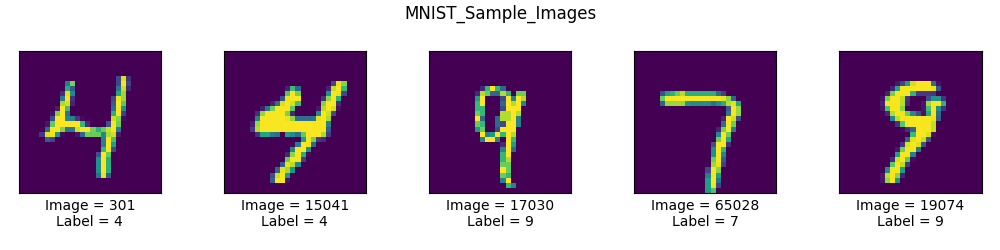
\includegraphics[scale=0.5]{images/MNIST_Sample_Images.png}\end{center}
	\caption{MNIST Sample Images}\label{MNISTFig}
\end{figure}

\subsubsection{notMNIST Dataset}
The notMNIST dataset consists of approximately 500k training and 19k test $(28,28,1)$ images of the characters `a' through `j' (see \Cref{notMNISTFig}). These characters are typeset with a wide variety of fonts. The training set has a roughly 6.5 percent misclassification rate, while the test set has a roughly 0.5 percent misclassification rate. Training against this dataset serves three functions: there are some additional challenges (memory constraints) involved in training a dataset of this size on a GPU, it appears to be a harder task than the MNIST classification problem, and it would be nice to see if our methods have a positive side effect on classifying problems with noisy and incorrect data. As such, we have made no attempt to clean up the data. Even without cleaning the data, we are still able to obtain error rates around 1.5\%, which, since it appears that researchers have not seriously attempted to benchmark this dataset, might be state of the art.

\begin{figure}[H]
	\begin{center} 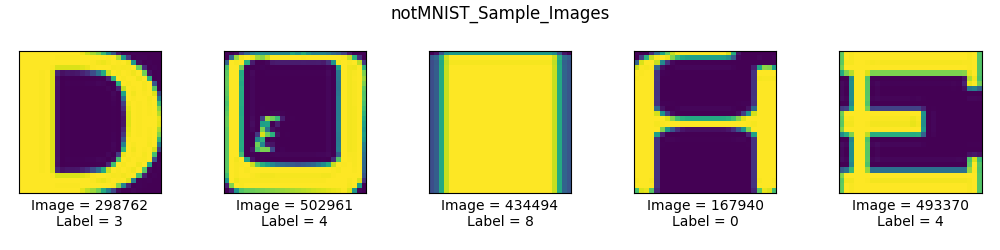
\includegraphics[scale=0.5]{images/notMNIST_Sample_Images.png}\end{center}
	\caption{notMNIST Sample Images}\label{notMNISTFig}
\end{figure}

\subsubsection{CIFAR10}
The CIFAR10 dataset consists of 50k training and 10k test $(32, 32,3)$ images pulled from 10 categories (e.g., cat, dog, etc.) (see \Cref{CIFAR10Fig}). This dataset is the most challenging of the three and is still used to benchmark state of the art models. Our best results yield error rates of around 20\%, which was state of the art in 2011, but far worse than what I expected to obtain with these models (see \Cref{rem:CIFAR10}).

\begin{figure}[H]
	\begin{center} 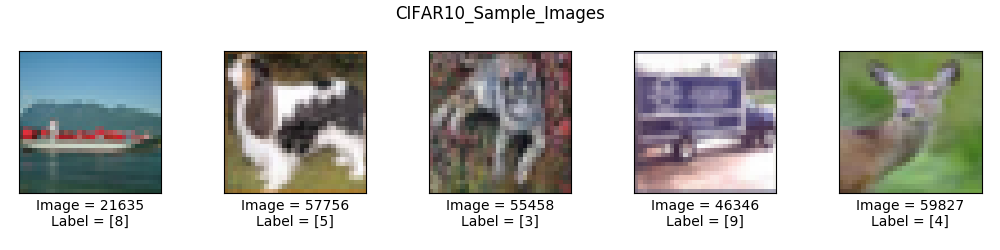
\includegraphics[scale=0.5]{images/CIFAR10_Sample_Images.png}\end{center}
	\caption{CIFAR10 Sample Images}\label{CIFAR10Fig}
\end{figure}

One reason for choosing image classification benchmarks is that it has been shown that deep networks are especially suitable for such problems, yet it is desirable to obtain faster models at the inference stage.

\subsubsection{Further discussion}
All of these datasets are available for free online, and our provided code automatically downloads the datasets and puts them into the required format for our models. 

\subsection{Exploratory visualization}
% Have you visualized a relevant characteristic or feature about the dataset or input data?
% Is the visualization thoroughly analyzed and discussed?
% If a plot is provided, are the axes, title, and datum clearly defined?
\begin{figure}
\centering
\begin{subfigure}{0.45\textwidth}
	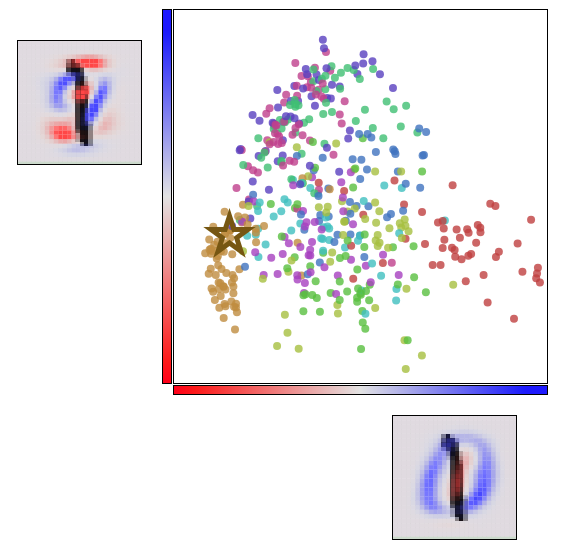
\includegraphics[width=\textwidth]{images/PCA1.png}
	\caption{An MNIST `1'}
\end{subfigure}
\begin{subfigure}{0.45\textwidth}
	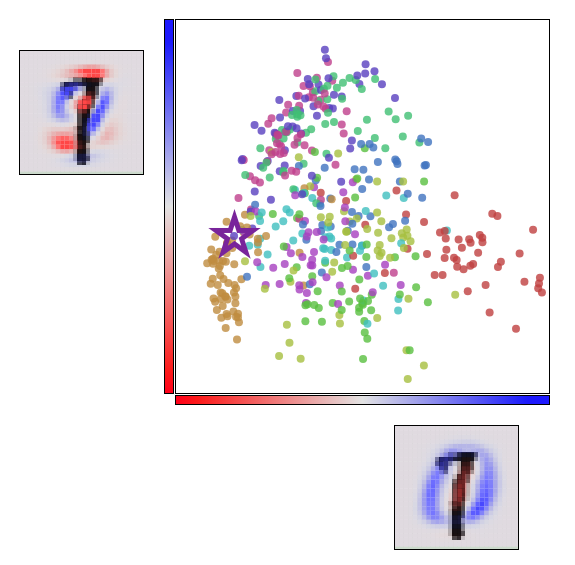
\includegraphics[width=\textwidth]{images/PCA7.png}
	\caption{An MNIST `7'}
\end{subfigure}
\caption{Similar MNIST images with distinct classifications.}\label{Fig:Similar}
\end{figure}
To illustrate our discussion from \Cref{sec:collab}, we consider the MNIST dataset and perform a principal component projection to $\mathbb{R}^2$. This projection is chosen so that the projection to $x$-axis  from the original dataset has the greatest variance in its image, while the projection to the $y$-axis produces the greatest variance in its image when restricted to the kernel of the projection to the $x$-axis. More informally this projection is chosen to spread out the data points as much as possible by maximizing the variance.

We have shamelessly stolen the visualization in \Cref{Fig:Similar} from Chris Olah's blog \cite{VisMNIST}. Each of the subfigures contains an image of the 2D PCA projection of a subset of the MNIST dataset. In each of the two images we have drawn attention to a different datapoint (indicated by a star). These two points are very close to each other in the projection (and they are visually quite similar) although they correspond to samples with different classifications.  One of the themes of this project is that a learned embedding which properly encodes the visual structure should also map these two points to relatively nearby points in unscaled logit space, but standardized supervised learning techniques will attempt to push these points as far as part as possible, as if the two images were radically different.

As a quick aside, let us explain what the images on the axes represent. On each axis is a copy of the corresponding sample image. Overlaid on this image is a heat map indicating the weight a pixel receives under corresponding principal component, with the shades of blue indicating how positive the corresponding weight is and the shades of red indicating how negative a weight is. In other words, each projection is given by a linear map $\mathbb{R}^{28\cdot 28}\to \mathbb{R}$ which we can regard as a 28 by 28 matrix which is then viewed as an image which we superimpose on the sample image. This allows us to see how much each pixel contributes to the corresponding projection.
\subsection{Algorithms and Techniques}
As mentioned above, all of our networks are modeled on the ResNet architecture \cite{ResNet}. We have made some minor variations to that model:
\begin{enumerate}
	\item We use the `pre-activation' order of operations as studied here \cite{Preactive}. This has been shown to improve the performance by a small amount.
	\item After each brick there is a halving in each spatial dimension and a doubling of the number of filters. In the published model this is performed by doing 1x1 convolutions with stride 2. Since this throws out 75\% of the learned data without regard to the values, we have replaced this with a 2x2 convolutions with stride 2 and valid padding. As a consequence, these reductions in spatial dimensions can only be performed on tensors  whose spatial dimensions are each divisible by 2.
\end{enumerate}

Our choice of using the ResNet architecture was based on two  reasons: 1) We wanted an architecture where it was straightforward to produce both deep and shallow variants and 2) we wanted an architecture which has been shown to have state of the art performance on competitive datasets.

\begin{remark}\label{rem:CIFAR10}
	Although the models I have trained all perform respectably on the given datasets, they are unable to match the state of the art performance on the CIFAR-10 dataset recorded in \cite{ResNet} (the error rates for my models trained with data augmentation was closer to 15\%, instead of the sub-10\% error rates they obtain). Examining implementations online of this architecture, it appears that there are quite a few subtleties that are left out of the paper and that replicating their results requires making some choices and may have depended on the implementations of the algorithms they used (e.g., see the comments in \cite{GitResnet}). 

	Another subtlety I noticed is that \cite{ResNet} appears to not be counting the huge number of learned parameters in the batch normalization layers. I was under the impression that one counts parameters for a couple of reasons: First, parameters are one source of memory constraints and second, the number of parameters indicates the ability of the model to memorize a dataset. If this is the goal, the batch normalization parameters need to be counted for, at least, the first reason. Depending on how the batch normalization is implemented (e.g., if it can learn the identity function), then it should also be counted for the second reason. 

	Most striking, none of the models that I ran into could be trained with the published learning rate of 0.1, which I found to be far too high to be stable. 
\end{remark}
We will discuss the choices of hyperparameters in the implementation section. 

% In this section, you will need to discuss the algorithms and techniques you intend to use for solving the problem. You should justify the use of each one based on the characteristics of the problem and the problem domain. Questions to ask yourself when writing this section:

% Are the algorithms you will use, including any default variables/parameters in the project clearly defined?
% Are the techniques to be used thoroughly discussed and justified?
% Is it made clear how the input data or datasets will be handled by the algorithms and techniques chosen?
\subsection{Benchmark}

As already indicated, we will test the performance of our collaboratively trained models against the benchmark set by the individual models when trained in an ensemble using the standard summary statistics (value of the cost/loss function and the error).  The ensemble benchmark will give us reference values for how well the models perform when trained individually. We will then compare this to how the models perform when we add the collaboration learning steps.
% In this section, you will need to provide a clearly defined benchmark result or threshold for comparing across performances obtained by your solution. The reasoning behind the benchmark (in the case where it is not an established result) should be discussed. Questions to ask yourself when writing this section:

% Has some result or value been provided that acts as a benchmark for measuring performance?
% Is it clear how this result or value was obtained (whether by data or by hypothesis)?

\section{Methodology}
Before diving into the details of our methods we would like to point to a fact of life which has become clear to us, while preparing this project. 
\begin{axiom}\label{ouraxiom}
	Training deep neural networks is time consuming and expensive. 
\end{axiom}

\Cref{ouraxiom} comes from the author's experience of spending \$175 on Amazon web services to train these models. Roughly half of this was spent on tuning and debugging and the other half was spent training the final models which took 3 days on a P2xlarge instance (my first runs on G2 instances were prone to crashing due to the limited GPU memory, although this was most likely due to a bug that was later corrected). While many of our design decisions are probably suboptimal, they can typically be explained by \Cref{ouraxiom}.

\subsection{Data Preprocessing}
Each of the models we have used begins with a batch normalization layer, which eliminates the need to normalize our data in advance. However there are still a few preprocessing steps we have implemented:
\begin{enumerate}
	\item We have shuffled all of our samples ahead of time. In the CIFAR10 and MNIST datasets we shuffled both the training and test sets together to ensure an even distribution across both. In the case of the notMNIST dataset, the test set has been cleaned ahead of time and has a drastically reduced misclassification rate. We would like to evaluate the effect of collaboration methods on noisier data so we have retained this property of the dataset.

	% \item The MNIST and notMNIST datasets are rescaled to 32x32. This both ensures that the all of the models have the same width and also makes it easier to implement our spatial dimension reductions using 2x2 convolutions with stride 2 (this requires each of the spatial dimensions to be divisible by $2^B$ where $B$ is the number of bricks in the model).

	\item In order to preclude additional obfuscating factors, we did not perform data augmentation, although this seems to be critical for reaching state of the art performance. 
	% \item We perform online data augmentation. On all of the datasets we perform random horizontal and vertical shifts of up to 4 pixels in each direction. On the CIFAR10 dataset we also allow random horizontal flips. The computational cost of online data augmentation was relatively low compared to the cost of training and has been shown to yield modest improvements in generalization error. 

	% More importantly, we have run into a rather special problem when training two models of varying depth simultaneously, measures need to be taken to ensure that one model does not drastically overfit before the other model has had a chance to learn the data. Data augmentation significantly reduces the ability of these models to overfit.

\end{enumerate}
\section{Implementation}
\subsection{Code structure}
We have implemented this project in Python using Tensorflow 1.1. We have written our own implementation of the above mentioned variation of the ResNet architecture. Because of the need to run so many different models and, at least during parameter tuning, to test against so many different choices of parameters we needed to write a Model class that encompassed many of the variations that we needed to consider. Each model consists of a Tensorflow graph for a given neural network, a reference to a batch manager class, and commands to train the network, gather the statistics, and arrange for the statistics to be logged by Logger classes. The model's train functions perform regular backups of model checkpoints and pickles the accumulated statistical data.

The relatively short implementation of the ResNet network is contained in the `resnet.py' file. The batch manager class gives the input pipeline and returns transformed batches. 

The Logger class is responsible for logging and pickling data, as well as logging checkpoints. While the Model is responsible for generating statistics (cross entropy, error rate), the logger is responsible for storing this data in numpy arrays, generating pyplot graphs, and writing this data to disk at the end of each epoch. We wanted to compare both training and test statistics over the course of training, but we did not want to evaluate the entire test set on each batch, so we only provide statistics from the end of each epoch. The reported error rate is the error rate over that epoch and the reported cost is the average cost over that epoch. This produces significantly smoother graphs than one would normally see if we logged every batch. 

\begin{remark}
Since the model is changing after each batch. It did not seem appropriate to average the statistics for the training data over each epoch. Instead we perform a running weighted average over each epoch. This provides better estimates in the early epochs when the model's performance is rapidly improving. However on the MNIST dataset, the models eventually approximate state of the art performance and can run into long streaks of perfect predictions which cause the model to incorrectly return 0\% error rates. In hindsight, I would have used statistics that were averaged over each epoch. We did not do this because of \Cref{ouraxiom}.
\end{remark}

The Model class has two subclasses: SingleModel and EnsembleModel. The SingleModel runs a single model and is a simplified form of the EnsembleModel which can train multiple models on the same task with or without collaboration. 

The datasets file includes code for downloading, preprocessing, and generating sample images from the datasets. The code for handling the notMNIST dataset is directly taken from the Tensorflow example code and is not due to myself. 

Finally, the analysis file gathers the pickled files, unpickles them, and stores the relevant data in a pandas dataframe. There are also additional functions which generate the graphs and tables from the appendices.

\subsection{Hyperparameters}
One of the special challenges of this proposal was finding choices of hyperparameters that work reasonably well on both shallow and deep models. We have chosen to use L2 weight decay set to $0.0001$ to further prevent potentially disastrous overfitting. We have also implemented a fairly simple learning rate scheduler: Once we are 50\% through the training we cut the learning rate in half, we do this again at 75\% and 90\% of the training is completed. I was a bit surprised to see that cutting the learning rate had such a positive effect when used with the adaptive momentum optimizer (Adam) which dynamically adjusts the learning factors for each variable, but the effect is noticeable (one can see the drops in error rates at these spots). These cuts allow the optimizer to explore smaller crevices in the cost function graph and seem to improve the performance of the model.

\begin{remark}
	The standard approach to learning rate scheduling is to pass a learning rate variable to the initialization of the optimizer and update this variable after each time step. However, in the case of the AdamOptimizer implementation in Tensorflow this causes the internal variables of the optimizer to be reinitialized after every time step and any learned momentum values to be lost. This drastically reduces the effectiveness of the optimizer. 

	We discovered that this effect can be avoided, by passing the learning rate to the optimizer as a placeholder value and not a variable.
\end{remark}

All models were trained on mini-batches of size 64. We settled on this choice as the smallest mini-batch size that yielded relatively low variance cost and error statistics. 
\begin{remark}
	One potential source of the discrepancy between the performance of our models and the published reports of \cite{ResNet} is that they use mini-batches of size 256 (divided over 8 GPUs)
\end{remark}

For our collaborative ensembles $\{ST, M\}$, with logit (resp.~softmax prediction) values on a sample $x$ denoted by $l_i(x)$ (resp.~$p_i(x)$), we considered the following collaborative cost functions: 
\begin{itemize}
	\item Symmetric cross entropy: \[SCE(x)=-\sum_{i=0}^{10} (p_i^{ST}(x) \log p_i^M(x) + p_i^{M}(x)\log p_i^{ST}(x))\]
	\item Sum of squares distance: \[ L2(x)= \sum_{i=0}^{10} (l_i^M(x)-l_i^{ST}(x))^2\]
	\item Manhattan distance: \[ L1(x)= \sum_{i=0}^{10} |l_i^M(x)-l_i^{ST}(x)|\]
\end{itemize}
Sorry to spoil the surprise, but we chose to use the symmetric cross entropy function rather than the ordinary cross entropy because it is symmetric. This is more than mathematical aesthetics. Even though minimizing the cross-entropy function would push the models to come to a consensus, gradient descent will adjust the parameters of a model differently depending on whether or not we consider it to be the first or the second model. Symmetrizing the cross-entropy resolves this issue.
% Note that we consider the symmetric cross entropy instead of the ordinary cross entropy to ensure that the gradients applied to each of the models are commensurable: Let $f(x)= -g(x)\log(h(x))$ then $\frac{\partial f}{\partial g}=-\log(h(x))$ which, for example, is 10 when $h(x)=e^{-10}$. In contrast, $\frac{\partial f}{\partial h} = \frac{-g(x)}{h(x)}$ which is $-e^{10}g(x)$. So even when $g(x)=h(x)=e^{-10}$, the gradients differ in absolute value by an order of  magnitude. 

One reason to consider the sum of squares distance is that the gradient is proportional to the difference between the logits. So as the difference approaches zero the magnitude of the gradient decreases which will give the models a bit more room to try to match the hard prediction labels. While the Manhattan distance always has a gradient which is a unit multiple of the derivative of the logits (except when the distance is zero and the derivative is not uniquely defined).

We scale all of our collaboration costs functions by a hyperparameter $\alpha \in \{0.0001, 0.01, 0.1, 1.0\}$ called the collaboration weight and trained the following variations of our ensembles:
\begin{enumerate}
	\item Standard ensemble of ST and M models.
	\item Collaborative ensemble of ST and M models ($\alpha \in \{0.0001, 0.01. 0.1, 1.0\}$):
	\begin{enumerate}
		\item Collaborative cost function = $\alpha \cdot SCE$.
		\item Collaborative cost function = $\alpha \cdot L2$.
		\item Collaborative cost function = $\alpha \cdot  L1$.
	\end{enumerate}
\end{enumerate}

Since each ensemble consists of two models and we additionally consider 3 different collaborative cost functions, each with one of four values of $\alpha$, we have to train $13$ different ensembles which in total involves training 26 models per dataset. We have to do this for each of the three datasets, which means we have to train 78 convolutional neural networks (see \Cref{ouraxiom}).

For the MNIST and CIFAR10 datasets we trained each model for 30 epochs. On the notMNIST dataset we only trained for 15 epochs. Both of these decisions were based on \Cref{ouraxiom}. I believe that there would be further gains if we trained longer since the Resnet models were trained for 3 times as long in \cite{ResNet} on the CIFAR10 dataset.
% In this section, the process for which metrics, algorithms, and techniques that you implemented for the given data will need to be clearly documented. It should be abundantly clear how the implementation was carried out, and discussion should be made regarding any complications that occurred during this process. Questions to ask yourself when writing this section:


% Is it made clear how the algorithms and techniques were implemented with the given datasets or input data?
% Were there any complications with the original metrics or techniques that required changing prior to acquiring a solution?
% Was there any part of the coding process (e.g., writing complicated functions) that should be documented?

% In this section, all of your preprocessing steps will need to be clearly documented, if any were necessary. From the previous section, any of the abnormalities or characteristics that you identified about the dataset will be addressed and corrected here. Questions to ask yourself when writing this section:

% If the algorithms chosen require preprocessing steps like feature selection or feature transformations, have they been properly documented?
% Based on the Data Exploration section, if there were abnormalities or characteristics that needed to be addressed, have they been properly corrected?
% If no preprocessing is needed, has it been made clear why?

\subsection{Refinement}
In the process of preparing the final models, we went through an extensive debugging and parameter tuning cycle. Debugging neural networks can be quite tricky, because broken code may not manifest itself except after extensive training, or it may just produce models that work, but not as well as they are supposed to. For example, a misplaced addition when composed with batch normalization can reduce the effectiveness of a model and cause the error rate to be at least 5 points higher \cite{Preactive}.  As another cautionary tale, we will mention that a misaligned tab caused our models to have about half as many layers; just enough to get acceptable performance, but quite short of what was expected. 

Here are a few other lessons that I learned in the refinement process which are all closely related to \Cref{ouraxiom}:
\begin{enumerate}
	\item Set random seeds. When making changes it is helpful if you can distinguish your changes from random chance.
	\item Unless absolutely necessary, debug with severely truncated datasets. If a bug is going to show up when your learning rate drops on the 30th epoch, it is best if you can see this in less than a day.
	\item Construct a simple model that is fast to train and obtains okay results and use this to debug the remainder of the code.
	\item Test your image classifiers on MNIST. If your error rate is above 3\%, than something is probably wrong.
	\item Use name scopes and Tensorboard. Visualizing the computational graph is quite useful for debugging. 
\end{enumerate}

I will now mention a couple of the hyperparameters that were tuned in the early phase of this project. First we needed to establish the architectures for the shallow and thin (ST) model and the medium (M) model. We also needed to establish an acceptable mini-batch size. Both of these decisions were heavily influenced by \Cref{ouraxiom}.

For the first task we wanted to find a shallow and thin model that was still able to obtain reasonable performance on the benchmarks (e.g., an error rate below 3\% on MNIST) so that this model would have some hope of aping the more complex model. With the Resnet architecture it is easy to adjust the width and depth as mentioned above. Experiments with a starting filter depth of 4 ($F=4$) showed that the model performed poorly regardless of the depth of the network, which is understandable for two simple reasons:
\begin{enumerate}
	\item The first convolutional layer only has 4 filter dimensions to map into. If the layer is supposed to reconstruct the image exactly and we have a color image (so 3 filters to begin with) this only leaves one independent dimension for a learned feature and minimal room to move the points in the sample space. 
	\item Because the model's penultimate layer has dimension 32, this yields a fairly constrained space to construct the linearly embedding $\mathbb{R}^{32}\to \mathbb{R}^{10}$ to the unscaled logits which separates the classes. 
\end{enumerate}
Experiments with a feature depth of 8, yielded reasonable results, so we used this for the ST model and doubled it for the M model. The models from \cite{ResNet} use 3 bricks ($B=3$), so we decided to follow their lead and use this for both models. This only left the choice of how many convolutional layers to include in each brick which is encoded in the choice of $R$. We settled on $R=1$ and $R=2$ for the ST and M models respectively\footnote{Although one can argue that a CNN with 10 convolutional layers is not `shallow', this is probably a matter of perspective. It is definitely shallower than the 50+ layer models that are now in use.}. Again this choice was primarily dictated by \Cref{ouraxiom}; it would have made more sense to have set $R$ to be at least 5 for the medium model, if we were to expect near state of the art results. 

In order to reduce the training time (see \Cref{ouraxiom}), we experimented with very small mini-batches, working our way up from 16, by powers of 2. The small mini-batches worked, but produced extremely noisy statistics and we eventually settled on a mini-batch size of 64. 

Do to \Cref{ouraxiom}, we did not retrain the entire collection of 78 neural networks during this fine tuning process, so we do not have comparable data to relate initial and final solutions. 
% In this section, you will need to discuss the process of improvement you made upon the algorithms and techniques you used in your implementation. For example, adjusting parameters for certain models to acquire improved solutions would fall under the refinement category. Your initial and final solutions should be reported, as well as any significant intermediate results as necessary. Questions to ask yourself when writing this section:

% Has an initial solution been found and clearly reported?
% Is the process of improvement clearly documented, such as what techniques were used?
% Are intermediate and final solutions clearly reported as the process is improved?
\section{Results}
\subsection{Model evaluation and validation}
After we trained our 78 models we have generated a lot of data which was pickled and squirreled away into 39 files. In the analysis file we gather the pickle data and store it in a single pandas data frame to make it easy to slice up for our analysis. Since we have considered 3 different collaboration methods, each with 4 possible collaboration weights, on 3 different datasets, we will do a preliminary analysis to see which combinations of collaboration methods and weights produced the best outcomes in terms of test error. We will then proceed with a more detailed analysis of the better performing collaborative models. 

Since we are considering so many models simultaneously we will focus our graphs and hence our attention on the final 10 training epochs and near the best performing models. The collaboratively trained models are all drawn in color and the traditionally trained models are in shades of gray.

We begin by considering the performance on the MNIST dataset in \Cref{STMNISTFig,MMNISTFig} which is located in the appendix. The careful reader will notice that there are not enough lines on the charts for the `L2' and `L1' collaborative models. This is because these models with collaboration weight $\alpha=1$ did poorly enough that they do not show up on these graphs\footnote{Adjusting the limits of the graphs to include these extra lines, made the graphs illegible.}. This illustrates that with large collaboration weights, the training process will primarily focus on making the models collaborate instead of fitting the data. 

While this was expected, what was not expected is that this is not such a factor when we learn with the symmetric cross entropy method.  A plausible explanation for this is by examining the gradients of these different cost functions. The gradients with respect to the symmetric cross entropy functions involve a sum of two terms, the first term we calculated above. This adjusts a logit for the first model at a rate proportional to the difference of the two models predictions. The second term is proportional to $p_i^{(1)}(1-p_i^{(1)})\log p_i^{(2)}$, which will become very small as the first model becomes confident in its predictions. So if the model has become reasonably confident in its predictions, the first term will dominate and we see that the gradients are essentially proportional to the difference between the two predictions (which will always be less than 1). This is in contrast to the gradients with respect to the L2 collaboration method which will be proportional to the difference between the unscaled logits which, by examining the values of these logits, will generally be larger than the difference between the predictions. The L1 norm will always be adjusting the unscaled logits by a factor of $\pm 1$, which will again be larger in magnitude than the difference in the predictions. So the latter two collaboration methods typically emphasize collaboration more.

Looking over the charts in \Cref{STMNISTFig,MMNISTFig,STnotMNISTFig,MnotMNISTFig,STCIFAR10Fig,MCIFAR10Fig} and the tables in \Cref{MNISTTab,MNISTCTab,notMNISTTab,notMNISTCTab,CIFAR10Tab,CIFAR10CTab} (which are located in the appendix), there are a few important observations to make:
\begin{enumerate}
	\item Collaborative models usually outperform their traditionally trained counterparts: On \emph{every} dataset at least 2 (and often more) of the collaborative models obtained lower test error than their counterparts trained in isolation.
	\item The collaboratively trained ST models can closely approximate the traditionally trained M models. This allows us to get similar performance with 20\% as many parameters and a threefold speedup.
	\item The traditionally trained ensembles out perform each of their constituents (as expected) and these models can be closely approximated by a single medium depth model that was trained in collaboration (obtaining a noticeable improvement in both memory and runtime over the ensemble model).
	\item All three collaboration methods yield improvements provided the collaboration rate is not too large and even for very small collaboration weights, we will often see an improvement.
	\item For symmetric cross entropy a collaboration weight of approximately 1 does well. For L2 and L1 values between 0.01 and 0.1 generally do well.
\end{enumerate}

We will now further examine the collaborative model which generally yielded the best results: The L2 method with weight 0.01. We will examine the training behavior and see how the collaborative models perform with respect to overfitting.  Examining \Cref{FinMNISTFig,FinnotMNISTFig,FinCIFAR10Fig} in the appendix, we can make a few observations:
\begin{enumerate}
	\item Collaborative models have smoother learning curves than the traditionally trained models.
	\item On the MNIST dataset, the smoother learning curve appears to lead to better final results, By which we mean the model spends less time correcting for past mistakes.
	\item On the notMNIST dataset, whose training set has roughly a 6.5\% misclassification rate\footnote{As a consequence all models do better on the test set (which has a 0.5\% misclassification rate) than on the training set.}, we see that the collaborative models are noticeably more resistant to overfitting, while still obtaining comparable results.
	\item On the CIFAR10 dataset, the collaborative models have very similar learning curves on the training set compared to their traditionally trained counterparts, yet they outperform these models on the test set.
	\item The models in the collaborative ensembles have more similar performance characteristics than those in traditional ensembles (as one should expect).
	\item The performance of collaborative ensembles improves as the degree of the collaboration decreases. This makes sense since this will increase the variance in their predictions. But even with very low collaboration weights, the individual models still outperform their traditional counterparts, so the corresponding collaborative ensemble has better performance than the traditional ensemble.
\end{enumerate}
It appears that the collaborative learning has a noticeable regularization effect on the models which makes them more resistant to overfitting similar to ensembles (it is hard for distinct models to overfit the data so that they generate highly correlated responses on new data). This may also be the source of the smoothing for the learning curves as the collaborative models are forced to make parameter adjustments that produce similar outputs which constrains the optimization problem in a constructive way (but this is just speculation).
% In this section, the final model and any supporting qualities should be evaluated in detail. It should be clear how the final model was derived and why this model was chosen. In addition, some type of analysis should be used to validate the robustness of this model and its solution, such as manipulating the input data or environment to see how the model’s solution is affected (this is called sensitivity analysis). Questions to ask yourself when writing this section:

% Is the final model reasonable and aligning with solution expectations? Are the final parameters of the model appropriate?
% Has the final model been tested with various inputs to evaluate whether the model generalizes well to unseen data?
% Is the model robust enough for the problem? Do small perturbations (changes) in training data or the input space greatly affect the results?


\subsection{Justification}
We can see that for any of the above collaborative methods and most choices of weights our collaborative models modestly outperform traditionally trained ensembles. Since the only difference between the collaborative approach and the traditional approach is the choice of cost function, this performance enhancement comes at virtually no cost. The only restriction here, and it is an important one, is that it is necessary to optimize both all of the models in the collaborative ensemble simultaneously, which means all of the models need to fit into memory and this can be a significant constraint if we are trying to get multiple large networks to collaborate. On the other hand, it appears that collaboratively training a model with a much weaker model only \emph{improves} both models. So adding smaller models into a collaboration should only require a comparatively small increase in memory, but noticeable improvements in performance. % In this section, your model’s final solution and its results should be compared to the benchmark you established earlier in the project using some type of statistical analysis. You should also justify whether these results and the solution are significant enough to have solved the problem posed in the project. Questions to ask yourself when writing this section:

% Are the final results found stronger than the benchmark result reported earlier?
% Have you thoroughly analyzed and discussed the final solution?
% Is the final solution significant enough to have solved the problem?

\section{Conclusion}
\subsection{Free-Form Visualization}
\begin{figure}
	\begin{center} 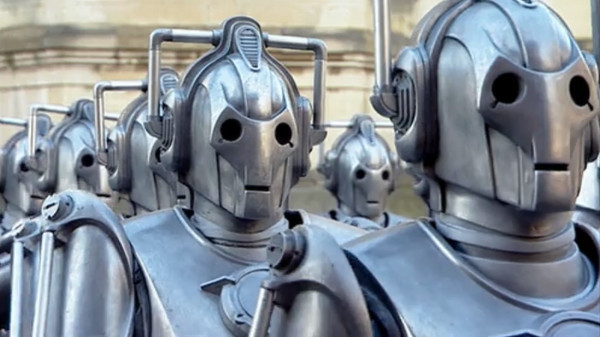
\includegraphics[scale=0.4]{images/cybermen.jpg}\end{center}
	\caption{Do not fear the collective.}\label{cybermen}
\end{figure}
Considering the above analysis, we conclude that are obvious and immediate benefits to training a collective of learning machines to solve a given task. If putting two neural networks together can produce such noticeable benefits, it is natural to ask what benefits we can get from ever larger and more varied collectives. After all, what is the worst thing that can happen (see \Cref{cybermen})?
% In this section, you will need to provide some form of visualization that emphasizes an important quality about the project. It is much more free-form, but should reasonably support a significant result or characteristic about the problem that you want to discuss. Questions to ask yourself when writing this section:

% Have you visualized a relevant or important quality about the problem, dataset, input data, or results?
% Is the visualization thoroughly analyzed and discussed?
% If a plot is provided, are the axes, title, and datum clearly defined?

\subsection{Reflection}
We have trained a large number of convolutional neural networks of varying depth under a variety of collaborative training methods. For most reasonable choices of hyperparameters these collaborative ensembles modestly outperform traditional ensembles on three publicly available datasets. Although the results of the collaborative ensembles are very close to those of the traditional ensembles, with many choices of hyperparameters, collaboratively trained \emph{individual} models outperform the traditionally trained counterparts by a more significant margin. This performance enhancement comes at virtually no cost provided that the computer has sufficient memory to train the models simultaneously. 

Developing a project on this scale has been quite educational. Training so many models, gathering all of the resultant data, and combining it into understandable representations has required quite a bit more work than the `quick-and-dirty' deep learning tutorials that one typically runs across. I have personally experienced the difficulty of fine-tuning of hyperparameters on this scale (see \Cref{ouraxiom}), as well as the manifold problems involved in debugging such networks. 

Although, I believe that this project would benefit from further study, I view at as a modest success. Although it does not appear that the deeper models learn any faster when trained collaboratively, they actually do improve by working with a weaker model. To the author, this is a surprise and warrants further investigation.
% In this section, you will summarize the entire end-to-end problem solution and discuss one or two particular aspects of the project you found interesting or difficult. You are expected to reflect on the project as a whole to show that you have a firm understanding of the entire process employed in your work. Questions to ask yourself when writing this section:

% Have you thoroughly summarized the entire process you used for this project?
% Were there any interesting aspects of the project?
% Were there any difficult aspects of the project?
% Does the final model and solution fit your expectations for the problem, and should it be used in a general setting to solve these types of problems?
\subsection{Improvement}
Now that we have identified reasonable collaboration methods and hyperparameters, it would be useful to further study these collaborative ensembles. For example:
\begin{enumerate}
	\item Do our results persist if we train the models for longer? If we add data augmentation?
	\item What happens if we change the collaboration weight over time? 
	\item What if we consider asymmetric collaborations where weaker models are forced to collaborate more than stronger ones?
	\item What happens when we make the ensembles larger? (The provided code is already designed for this generality)
	\item What happens when the ensembles consist of identical architectures? Do we still see such regularization effects?
	\item Can a Very deep model's performance be improved by working with such a shallow and thin model?
	\item We can easily separate the collaborative learning step from the training step. An important property of learning to collaborate is that \emph{it does not require labeled training data.} In principle, a collaborative ensemble can learn to come to a consensus on any unlabeled dataset, even random noise. It would be interesting to see if mixing collaborative training and traditional training can produce even better outcomes and whether it is actually important to feed in similar data for the learning process. 
\end{enumerate}

Given the limited range of hyperparameters considered and the limited training time, I am confident that these models could be improved upon. 
% In this section, you will need to provide discussion as to how one aspect of the implementation you designed could be improved. As an example, consider ways your implementation can be made more general, and what would need to be modified. You do not need to make this improvement, but the potential solutions resulting from these changes are considered and compared/contrasted to your current solution. Questions to ask yourself when writing this section:

% Are there further improvements that could be made on the algorithms or techniques you used in this project?
% Were there algorithms or techniques you researched that you did not know how to implement, but would consider using if you knew how?
% If you used your final solution as the new benchmark, do you think an even better solution exists?

% \section{Project Design}
% We will produce at least two models for image classification, using standard convolutional neural network techniques (Relu/elu/maxout activations, convolutional layers, average/max pooling, batch normalization). The hope is to find two models which can very closely fit the training data, but have rather different generalization error, speed, memory requirements, and rates of learning. While I do not want to commit to an exact implementation, given sufficient time I would like to construct some shallower and thinner ResNet models \cite{ResNet}. By varying the layers and feature depths of such models we should be able to construct two models with the desired characteristics. Experimentation indicates that with my limited computational facilities, I can only construct models with very similar generalization error rates and rates of learning under the constraint that the model eventually learns the training data, so I only want to commit to construct two models with sufficiently different computational requirements. 

% The general workflow model will be mostly standard, with some exceptions given our limited goal:
% \begin{enumerate}
% 	\item We will not preprocess the images by normalizing them because our model will use batch normalization at the bottom layer.
% 	\item We will not perform any data augmentation. With my resources, I do not expect to match any of the top models.
% 	\item We will write subroutines to generate training, validation, and test batches. 
% 	\item We will write subroutines for the building blocks of our models in tensorflow (or possibly Keras).
% 	\item We will write subroutines for generating each of our models.
% 	\item We will generate summary statistics (cost, cross entropy, accuracy) and write them to a file for later reference.
% 	\item We will test all models on truncated datasets and use tensorboard for debugging (if we use tensorflow). 
% 	\item We will run the model using a range of hyperparameters (in particular on the choice of cost function as elaborated above). 
% 	\item We will compare the performance of the individual models trained separately, trained together collaboratively, as an ensemble, and the weaker model trained against soft targets as in \cite{Distillation}.
% \end{enumerate}
% \section{Evaluation Metrics/Benchmark models}
% We will evaluate our models by accuracy with respect to the number of training steps/training time. Our benchmark models will consist of the individual models trained in a non-collaborative fashion. By construction, all of these metrics and benchmarks will be reproducible. 

% \section{Our models}
% Our models are based on the Resnet architecture \cite{ResNet}. This architecture consists of several bricks which end in a reduction in each of the two spatial dimensions by a factor of 2 and double the feature dimension, resulting in an overall increase in the feature space by a factor of 2. In the original resnet architecture this is done by performing a sequence of 2 3x3 convolutions, the first of which has stride 2 and summing the output with a `shortcut' which is a 1x1 convolution of stride 2. 

% Each of the bricks consists of $n$ iterations of the following: two 3x3 convolutions with the same number of features as the input are calculated and summed with a 
\bibliographystyle{alpha}
\bibliography{biblio}
\newpage
\appendix
\section{Comparison of methods and weights}
\subsection{Graphs}
\begin{figure}[H]
	\begin{center} 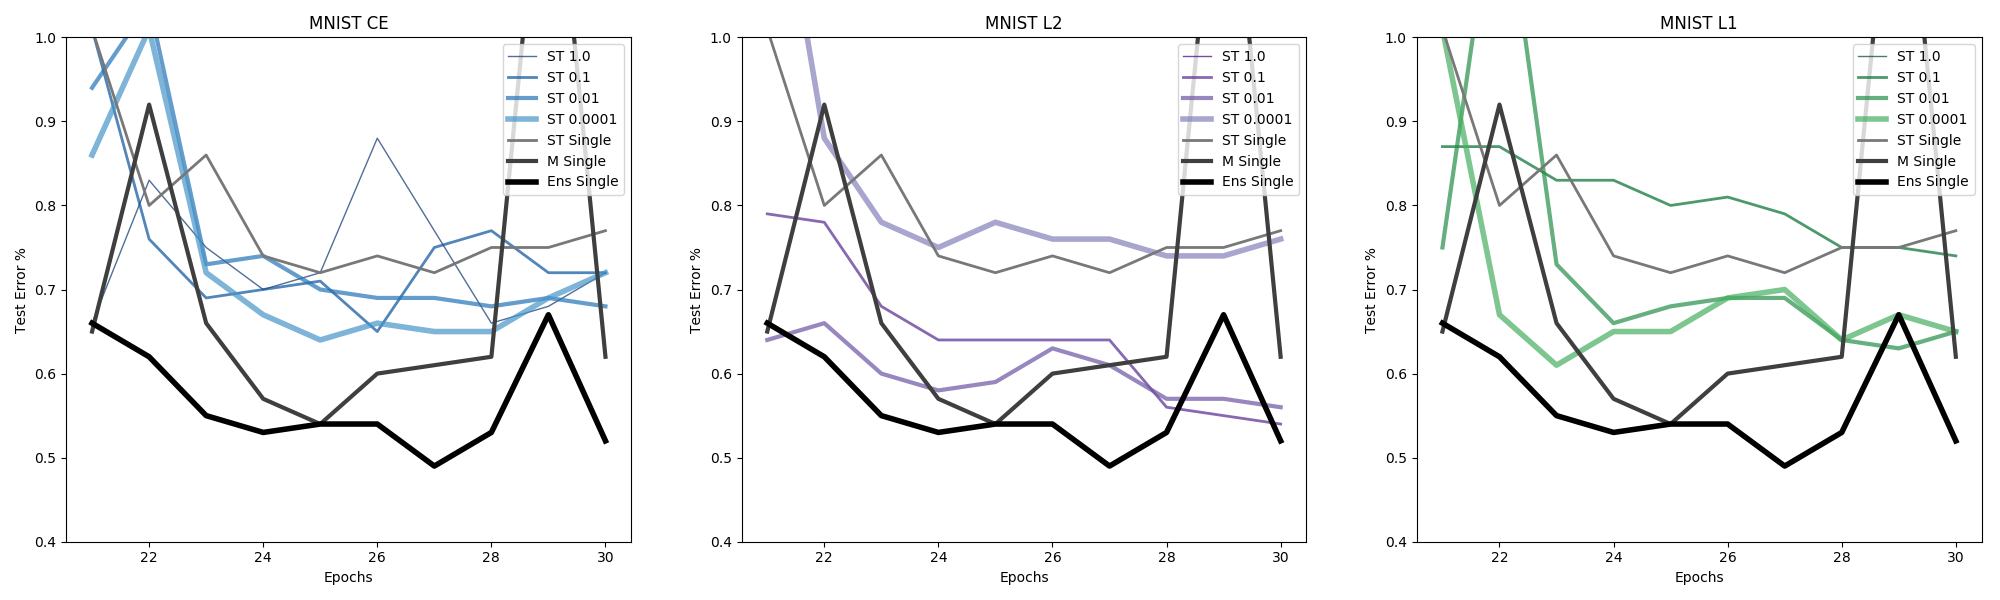
\includegraphics[scale=0.3]{graphs/MNIST_ST_TestError.png}\end{center}
	\caption{MNIST Shallow and thin models}\label{STMNISTFig}
\end{figure}
\begin{figure}[H]
	\begin{center} 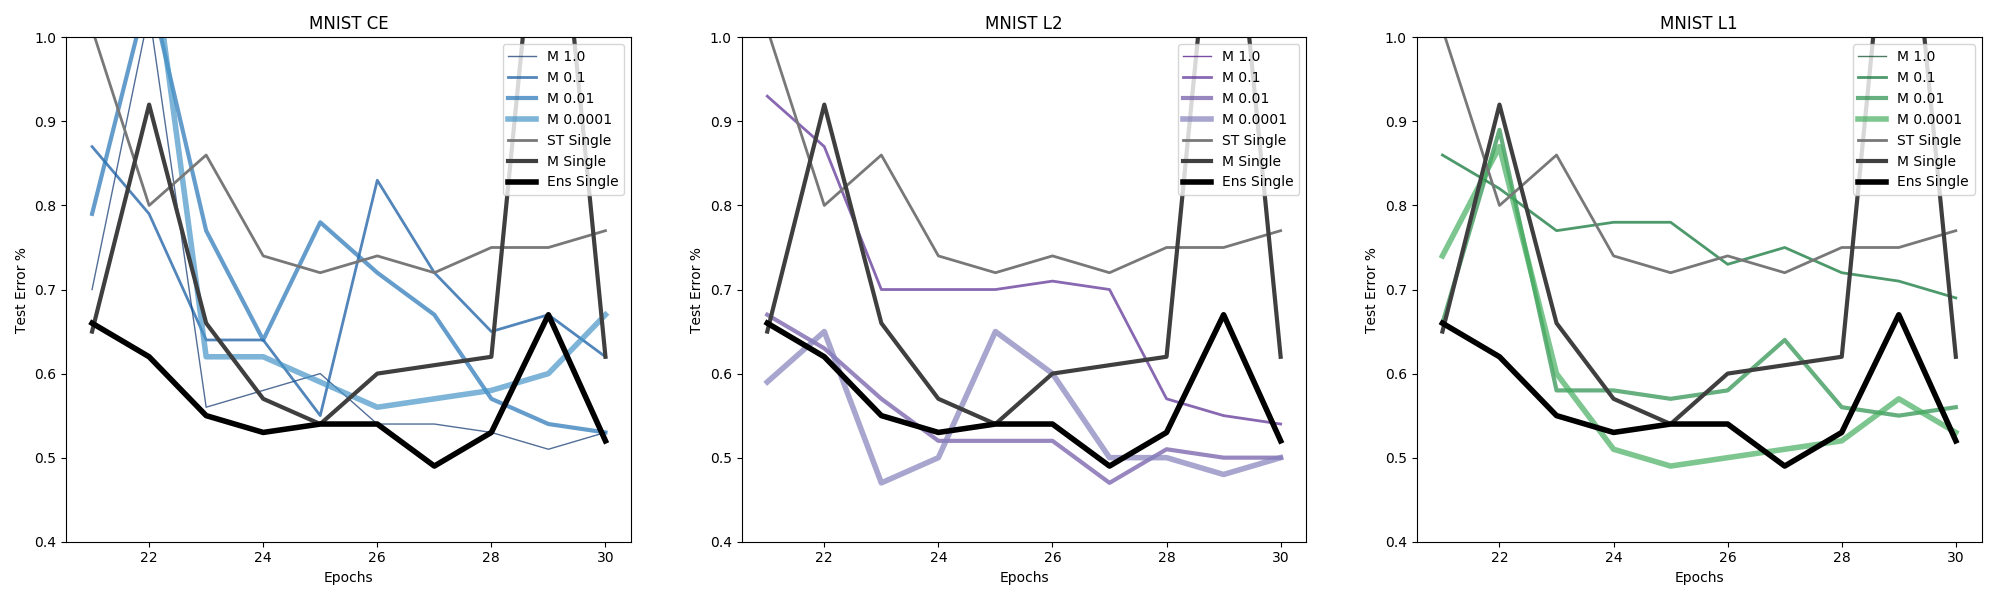
\includegraphics[scale=0.3]{graphs/MNIST_M_TestError.png}\end{center}
	\caption{MNIST Medium models}\label{MMNISTFig}
\end{figure}
\begin{figure}[H]
	\begin{center} 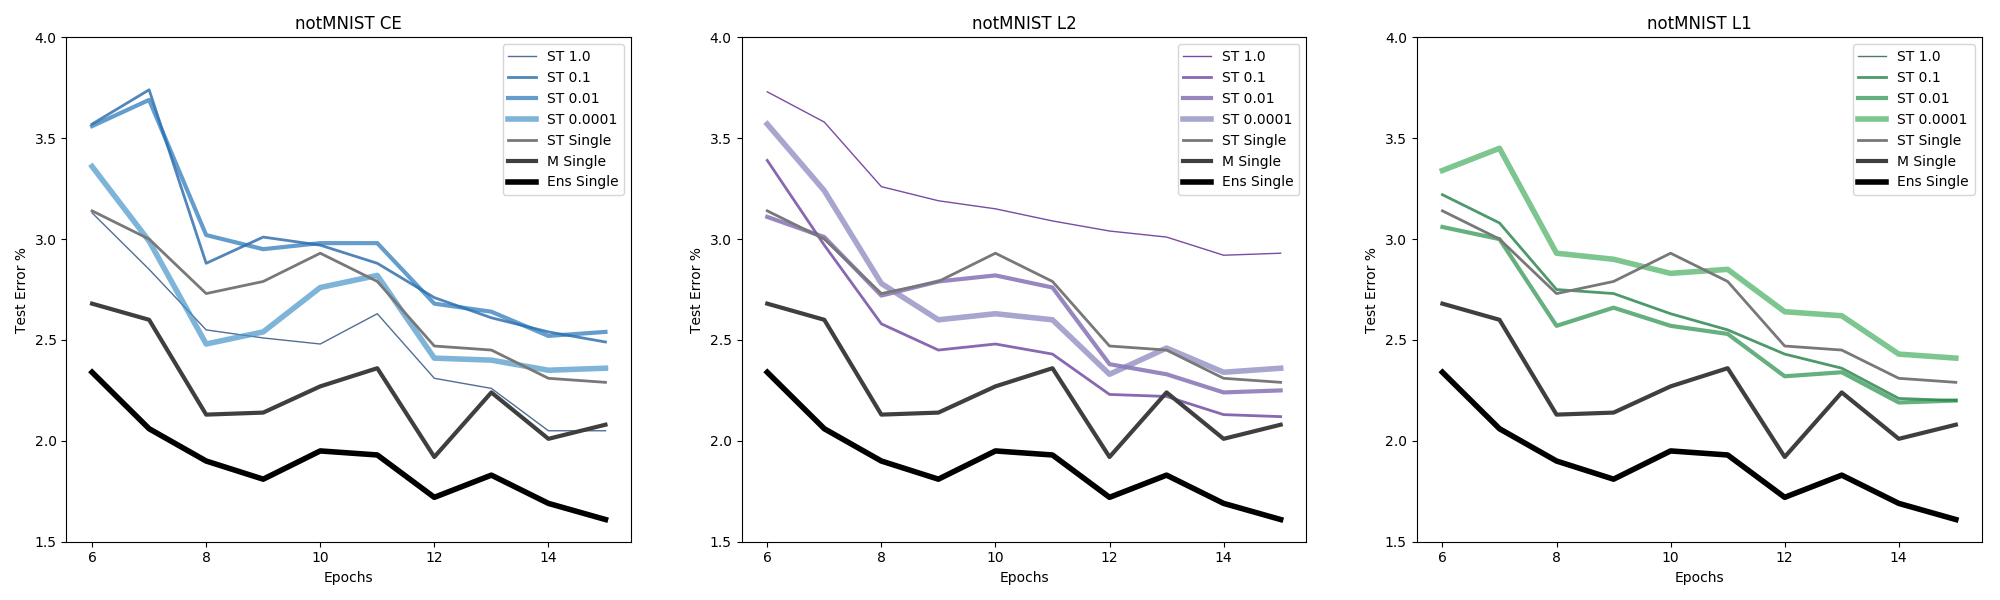
\includegraphics[scale=0.3]{graphs/notMNIST_ST_TestError.png}\end{center}
	\caption{notMNIST Shallow and thin models}\label{STnotMNISTFig}
\end{figure}
\begin{figure}[H]
	\begin{center} 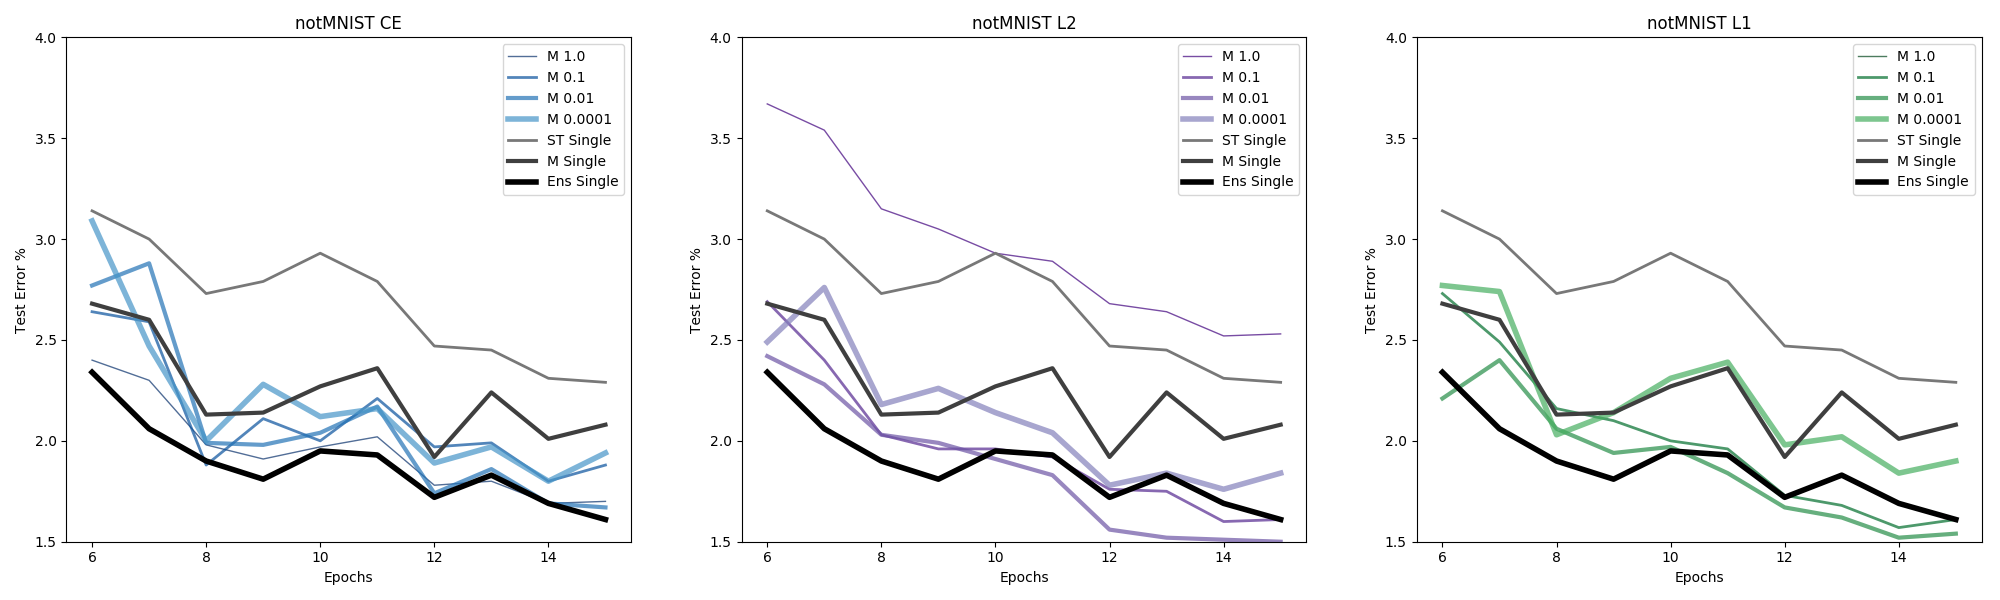
\includegraphics[scale=0.3]{graphs/notMNIST_M_TestError.png}\end{center}
	\caption{notMNIST Medium models}\label{MnotMNISTFig}
\end{figure}
\begin{figure}[H]
	\begin{center} 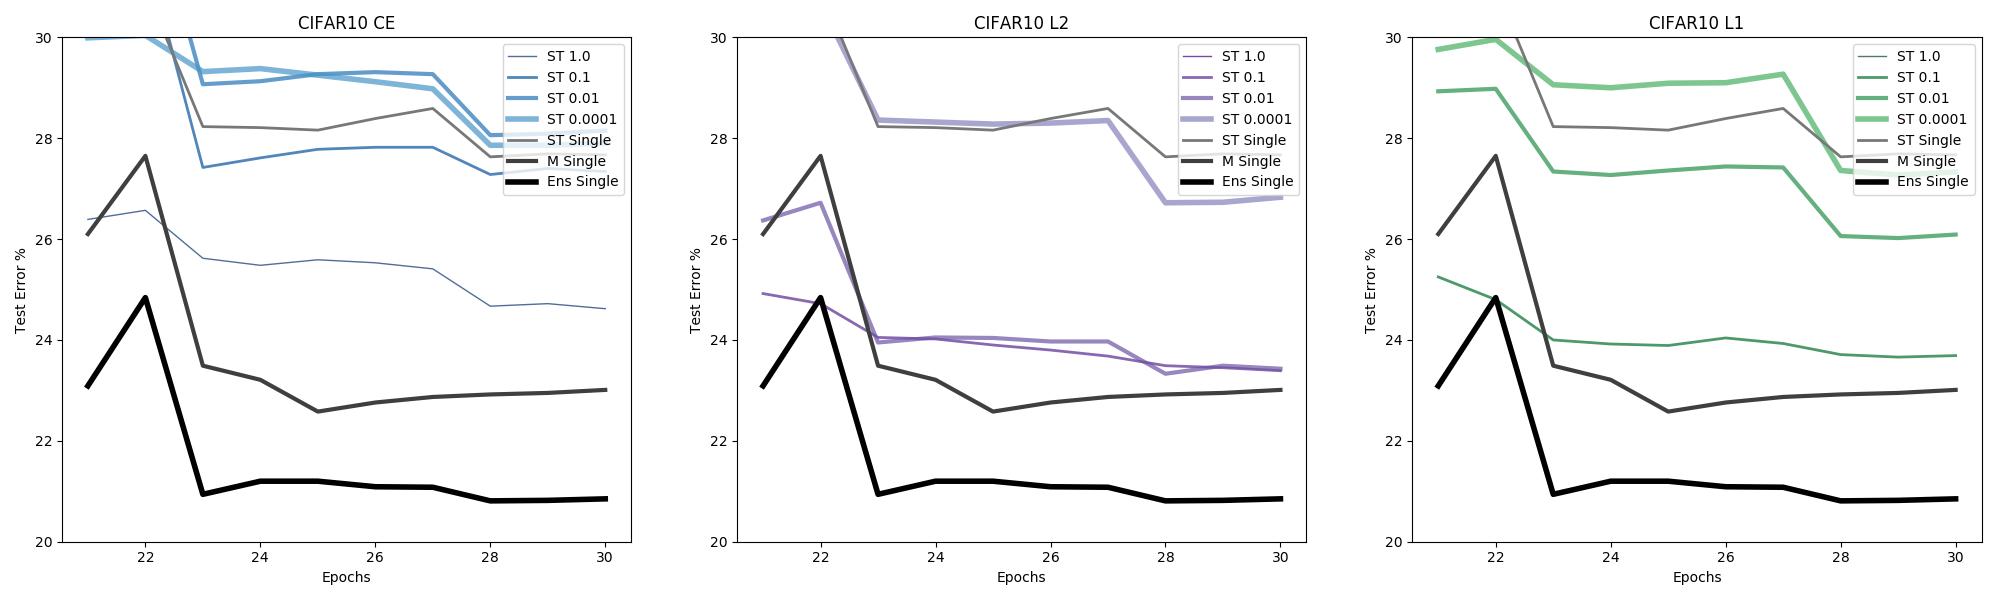
\includegraphics[scale=0.3]{graphs/CIFAR10_ST_TestError.png}\end{center}
	\caption{CIFAR10 Shallow and thin models}\label{STCIFAR10Fig}
\end{figure}
\begin{figure}[H]
	\begin{center} 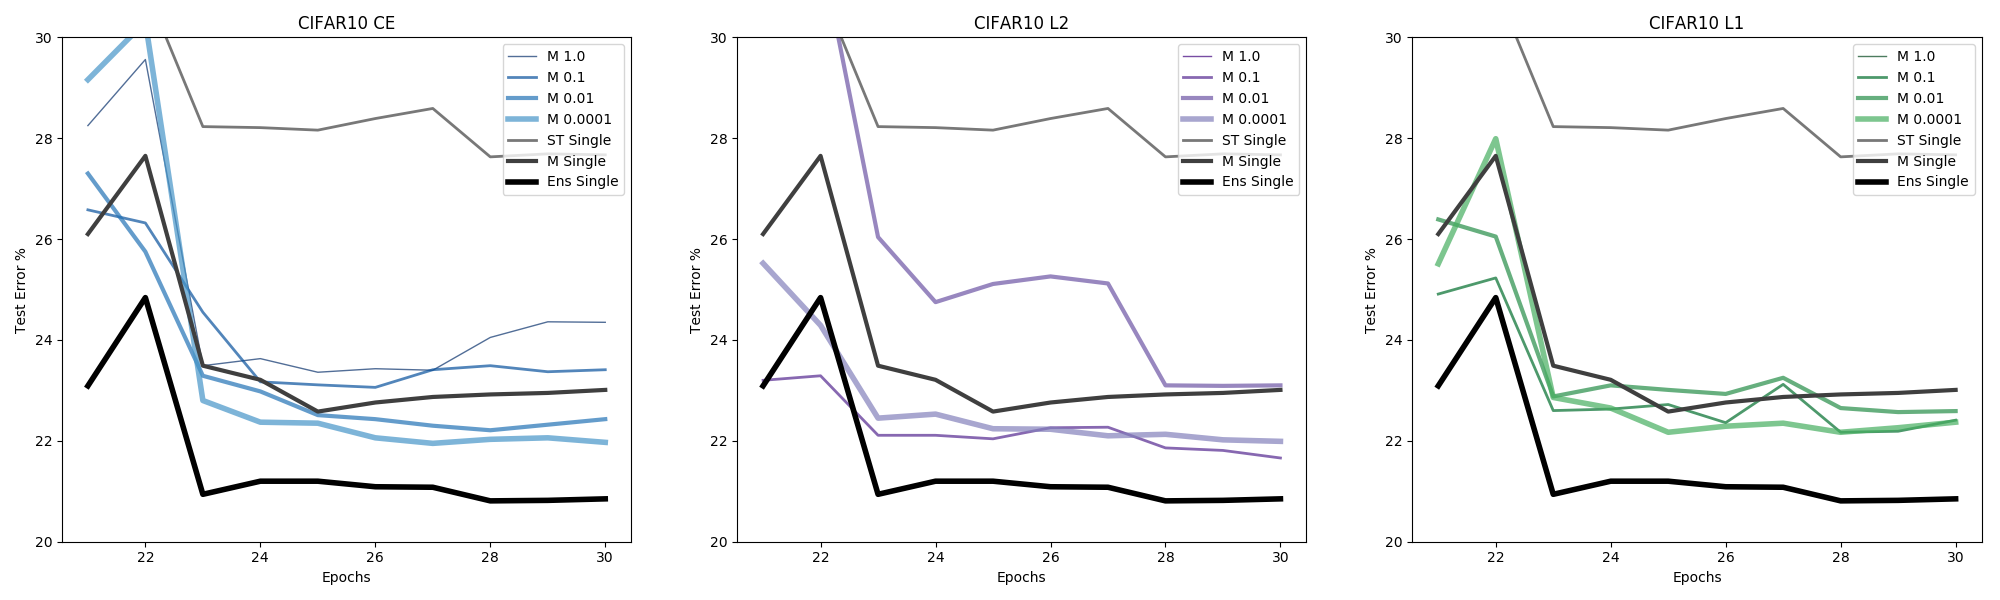
\includegraphics[scale=0.3]{graphs/CIFAR10_M_TestError.png}\end{center}
	\caption{CIFAR10 Medium models}\label{MCIFAR10Fig}
\end{figure}


\subsection{Tables}
Bold indicates best result. 
\begin{figure}[H]
\begin{center}
\begin{tabular}{lr}
\hline
 ST Model        &   Test Error \% \\
\hline
 ('CE', 1.0)     &           0.72 \\
 ('CE', 0.1)     &           0.72 \\
 ('CE', 0.01)    &           0.68 \\
 ('CE', 0.0001)  &           0.72 \\
 ('L1', 1.0)     &           2.75 \\
 ('L1', 0.1)     &           0.74 \\
 ('L1', 0.01)    &           0.65 \\
 ('L1', 0.0001)  &           0.65 \\
 ('L2', 1.0)     &           1.38 \\
 ('L2', 0.1)     &           {\bf 0.54} \\
 ('L2', 0.01)    &           0.56 \\
 ('L2', 0.0001)  &           0.76 \\
 ('Single', 1.0) &           0.77 \\
\hline
\end{tabular}\begin{tabular}{lr}
\hline
 M Model         &   Test Error \% \\
\hline
 ('CE', 1.0)     &           0.53 \\
 ('CE', 0.1)     &           0.62 \\
 ('CE', 0.01)    &           0.53 \\
 ('CE', 0.0001)  &           0.67 \\
 ('L1', 1.0)     &           2.75 \\
 ('L1', 0.1)     &           0.69 \\
 ('L1', 0.01)    &           0.56 \\
 ('L1', 0.0001)  &           0.53 \\
 ('L2', 1.0)     &           1.33 \\
 ('L2', 0.1)     &           0.54 \\
 ('L2', 0.01)    &           {\bf 0.5}  \\
 ('L2', 0.0001)  &           {\bf 0.5}  \\
 ('Single', 1.0) &           0.62 \\
\hline
\end{tabular}\begin{tabular}{lr}
\hline
 Ens Model       &   Test Error \% \\
\hline
 ('CE', 1.0)     &           0.59 \\
 ('CE', 0.1)     &           0.54 \\
 ('CE', 0.01)    &           0.52 \\
 ('CE', 0.0001)  &           0.61 \\
 ('L1', 1.0)     &           2.74 \\
 ('L1', 0.1)     &           0.73 \\
 ('L1', 0.01)    &           0.59 \\
 ('L1', 0.0001)  &           0.53 \\
 ('L2', 1.0)     &           1.37 \\
 ('L2', 0.1)     &           0.56 \\
 ('L2', 0.01)    &           {\bf 0.5}  \\
 ('L2', 0.0001)  &           0.57 \\
 ('Single', 1.0) &           0.52 \\
\hline
\end{tabular}
\end{center}
\caption{MNIST Final Test Error Results}\label{MNISTTab}
\end{figure}

\begin{figure}[H]
\begin{center}
\begin{tabular}{lr}
\hline
 ST Model        &   Test Cost \\
\hline
 ('CE', 1.0)     &   0.034945  \\
 ('CE', 0.1)     &   0.0421644 \\
 ('CE', 0.01)    &   0.04444   \\
 ('CE', 0.0001)  &   0.0468188 \\
 ('L1', 1.0)     &   0.156449  \\
 ('L1', 0.1)     &   0.0410959 \\
 ('L1', 0.01)    &   0.0280316 \\
 ('L1', 0.0001)  &   0.0324634 \\
 ('L2', 1.0)     &   0.0729461 \\
 ('L2', 0.1)     &   0.0316807 \\
 ('L2', 0.01)    &   {\bf 0.0257211} \\
 ('L2', 0.0001)  &   0.0316473 \\
 ('Single', 1.0) &   0.0459429 \\
\hline
\end{tabular}\begin{tabular}{lr}
\hline
 M Model         &   Test Cost \\
\hline
 ('CE', 1.0)     &   0.026722  \\
 ('CE', 0.1)     &   0.0378052 \\
 ('CE', 0.01)    &   0.0440946 \\
 ('CE', 0.0001)  &   0.0480394 \\
 ('L1', 1.0)     &   0.179248  \\
 ('L1', 0.1)     &   0.0429026 \\
 ('L1', 0.01)    &   0.0220588 \\
 ('L1', 0.0001)  &   0.0300227 \\
 ('L2', 1.0)     &   0.0850099 \\
 ('L2', 0.1)     &   0.0308176 \\
 ('L2', 0.01)    &   {\bf 0.0197911} \\
 ('L2', 0.0001)  &   0.0261167 \\
 ('Single', 1.0) &   0.0388529 \\
\hline
\end{tabular}\begin{tabular}{lr}
\hline
 Ens Model       &   Test Cost \\
\hline
 ('CE', 1.0)     &   0.0191731 \\
 ('CE', 0.1)     &   0.0248691 \\
 ('CE', 0.01)    &   0.0294754 \\
 ('CE', 0.0001)  &   0.0329928 \\
 ('L1', 1.0)     &   0.137231  \\
 ('L1', 0.1)     &   0.0271439 \\
 ('L1', 0.01)    &   0.0183511 \\
 ('L1', 0.0001)  &   0.0218571 \\
 ('L2', 1.0)     &   0.0549106 \\
 ('L2', 0.1)     &   0.0200527 \\
 ('L2', 0.01)    &   {\bf 0.0168002} \\
 ('L2', 0.0001)  &   0.0201273 \\
 ('Single', 1.0) &   0.0286906 \\
\hline
\end{tabular}
\end{center}
\caption{MNIST Final Test Cost Results}\label{MNISTCTab}
\end{figure}

\begin{figure}[H]
\begin{center}
\begin{tabular}{lr}
\hline
 ST Model        &   Test Error \% \\
\hline
 ('CE', 1.0)     &           {\bf 2.05} \\
 ('CE', 0.1)     &           2.49 \\
 ('CE', 0.01)    &           2.54 \\
 ('CE', 0.0001)  &           2.36 \\
 ('L1', 1.0)     &           4.43 \\
 ('L1', 0.1)     &           2.2  \\
 ('L1', 0.01)    &           2.2  \\
 ('L1', 0.0001)  &           2.41 \\
 ('L2', 1.0)     &           2.93 \\
 ('L2', 0.1)     &           2.12 \\
 ('L2', 0.01)    &           2.25 \\
 ('L2', 0.0001)  &           2.36 \\
 ('Single', 1.0) &           2.29 \\
\hline
\end{tabular}\begin{tabular}{lr}
\hline
 M Model         &   Test Error \% \\
\hline
 ('CE', 1.0)     &           1.7  \\
 ('CE', 0.1)     &           1.88 \\
 ('CE', 0.01)    &           1.67 \\
 ('CE', 0.0001)  &           1.94 \\
 ('L1', 1.0)     &           4.31 \\
 ('L1', 0.1)     &           1.61 \\
 ('L1', 0.01)    &           1.54 \\
 ('L1', 0.0001)  &           1.9  \\
 ('L2', 1.0)     &           2.53 \\
 ('L2', 0.1)     &           1.61 \\
 ('L2', 0.01)    &           {\bf 1.5}  \\
 ('L2', 0.0001)  &           1.84 \\
 ('Single', 1.0) &           2.08 \\
\hline
\end{tabular}\begin{tabular}{lr}
\hline
 Ens Model       &   Test Error \% \\
\hline
 ('CE', 1.0)     &           1.67 \\
 ('CE', 0.1)     &           1.74 \\
 ('CE', 0.01)    &           1.61 \\
 ('CE', 0.0001)  &           1.61 \\
 ('L1', 1.0)     &           4.37 \\
 ('L1', 0.1)     &           1.78 \\
 ('L1', 0.01)    &           1.58 \\
 ('L1', 0.0001)  &           1.59 \\
 ('L2', 1.0)     &           2.7  \\
 ('L2', 0.1)     &           1.74 \\
 ('L2', 0.01)    &           {\bf 1.55} \\
 ('L2', 0.0001)  &           1.57 \\
 ('Single', 1.0) &           1.61 \\
\hline
\end{tabular}
\end{center}
\caption{notMNIST Final Test Error Results}\label{notMNISTTab}
\end{figure}

\begin{figure}[H]
\begin{center}
\begin{tabular}{lr}
\hline
 ST Model        &   Test Cost \\
\hline
 ('CE', 1.0)     &   0.0912072 \\
 ('CE', 0.1)     &   0.10222   \\
 ('CE', 0.01)    &   0.107765  \\
 ('CE', 0.0001)  &   0.0975916 \\
 ('L1', 1.0)     &   0.189134  \\
 ('L1', 0.1)     &   0.0967725 \\
 ('L1', 0.01)    &   0.0909284 \\
 ('L1', 0.0001)  &   0.103207  \\
 ('L2', 1.0)     &   0.119305  \\
 ('L2', 0.1)     &   0.0901654 \\
 ('L2', 0.01)    &   {\bf 0.0891081} \\
 ('L2', 0.0001)  &   0.0979867 \\
 ('Single', 1.0) &   0.0973864 \\
\hline
\end{tabular}\begin{tabular}{lr}
\hline
 M Model         &   Test Cost \\
\hline
 ('CE', 1.0)     &   0.0729853 \\
 ('CE', 0.1)     &   0.0886137 \\
 ('CE', 0.01)    &   0.10884   \\
 ('CE', 0.0001)  &   0.113915  \\
 ('L1', 1.0)     &   0.191429  \\
 ('L1', 0.1)     &   0.0726474 \\
 ('L1', 0.01)    &   0.0764119 \\
 ('L1', 0.0001)  &   0.106903  \\
 ('L2', 1.0)     &   0.113529  \\
 ('L2', 0.1)     &   0.0722657 \\
 ('L2', 0.01)    &  {\bf 0.0712102} \\
 ('L2', 0.0001)  &   0.100407  \\
 ('Single', 1.0) &   0.122331  \\
\hline
\end{tabular}\begin{tabular}{lr}
\hline
 Ens Model       &   Test Cost \\
\hline
 ('CE', 1.0)     &   0.0597912 \\
 ('CE', 0.1)     &   0.0566993 \\
 ('CE', 0.01)    &   0.0622045 \\
 ('CE', 0.0001)  &   0.0580449 \\
 ('L1', 1.0)     &   0.171096  \\
 ('L1', 0.1)     &   0.0675368 \\
 ('L1', 0.01)    &   {\bf 0.053546}  \\
 ('L1', 0.0001)  &   0.0596633 \\
 ('L2', 1.0)     &   0.10414   \\
 ('L2', 0.1)     &   0.0662774 \\
 ('L2', 0.01)    &   0.055066  \\
 ('L2', 0.0001)  &   0.056186  \\
 ('Single', 1.0) &   0.0619581 \\
\hline
\end{tabular}
\end{center}
\caption{notMNIST Final Test Cost Results}\label{notMNISTCTab}
\end{figure}

\begin{figure}[H]
\begin{center}
\begin{tabular}{lr}
\hline
 ST Model        &   Test Error \% \\
\hline
 ('CE', 1.0)     &          24.62 \\
 ('CE', 0.1)     &          27.34 \\
 ('CE', 0.01)    &          28.15 \\
 ('CE', 0.0001)  &          27.9  \\
 ('L1', 1.0)     &          45.74 \\
 ('L1', 0.1)     &          23.69 \\
 ('L1', 0.01)    &          26.09 \\
 ('L1', 0.0001)  &          27.33 \\
 ('L2', 1.0)     &          34.87 \\
 ('L2', 0.1)     &          {\bf 23.39} \\
 ('L2', 0.01)    &          23.43 \\
 ('L2', 0.0001)  &          26.83 \\
 ('Single', 1.0) &          27.67 \\
\hline
\end{tabular}\begin{tabular}{lr}
\hline
 M Model         &   Test Error \% \\
\hline
 ('CE', 1.0)     &          24.35 \\
 ('CE', 0.1)     &          23.41 \\
 ('CE', 0.01)    &          22.43 \\
 ('CE', 0.0001)  &          21.97 \\
 ('L1', 1.0)     &          45.12 \\
 ('L1', 0.1)     &          22.41 \\
 ('L1', 0.01)    &          22.59 \\
 ('L1', 0.0001)  &          22.37 \\
 ('L2', 1.0)     &          33.53 \\
 ('L2', 0.1)     &          {\bf 21.66} \\
 ('L2', 0.01)    &          23.1  \\
 ('L2', 0.0001)  &          21.99 \\
 ('Single', 1.0) &          23.01 \\
\hline
\end{tabular}\begin{tabular}{lr}
\hline
 Ens Model       &   Test Error \% \\
\hline
 ('CE', 1.0)     &          21.6  \\
 ('CE', 0.1)     &          20.85 \\
 ('CE', 0.01)    &          20.42 \\
 ('CE', 0.0001)  &          20.01 \\
 ('L1', 1.0)     &          45.42 \\
 ('L1', 0.1)     &          20.93 \\
 ('L1', 0.01)    &          20.86 \\
 ('L1', 0.0001)  &          20.16 \\
 ('L2', 1.0)     &          34.15 \\
 ('L2', 0.1)     &          21.12 \\
 ('L2', 0.01)    &          20.32 \\
 ('L2', 0.0001)  &          {\bf 19.72} \\
 ('Single', 1.0) &          20.85 \\
\hline
\end{tabular}
\end{center}
\caption{CIFAR10 Final Test Error Results}\label{CIFAR10Tab}
\end{figure}

\begin{figure}[H]
\begin{center}
\begin{tabular}{lr}
\hline
 ST Model        &   Test Cost \\
\hline
 ('CE', 1.0)     &    0.774816 \\
 ('CE', 0.1)     &    0.949555 \\
 ('CE', 0.01)    &    0.963046 \\
 ('CE', 0.0001)  &    0.957336 \\
 ('L1', 1.0)     &    1.31941  \\
 ('L1', 0.1)     &    0.704402 \\
 ('L1', 0.01)    &    0.843182 \\
 ('L1', 0.0001)  &    0.960852 \\
 ('L2', 1.0)     &    1.02301  \\
 ('L2', 0.1)     &    {\bf 0.696001} \\
 ('L2', 0.01)    &    0.706045 \\
 ('L2', 0.0001)  &    0.925666 \\
 ('Single', 1.0) &    0.96121  \\
\hline
\end{tabular}\begin{tabular}{lr}
\hline
 M Model         &   Test Cost \\
\hline
 ('CE', 1.0)     &    0.787899 \\
 ('CE', 0.1)     &    0.870409 \\
 ('CE', 0.01)    &    1.11529  \\
 ('CE', 0.0001)  &    1.77734  \\
 ('L1', 1.0)     &    1.33951  \\
 ('L1', 0.1)     &    0.705127 \\
 ('L1', 0.01)    &    0.826856 \\
 ('L1', 0.0001)  &    1.43472  \\
 ('L2', 1.0)     &    1.01763  \\
 ('L2', 0.1)     &    {\bf 0.689528} \\
 ('L2', 0.01)    &    0.766554 \\
 ('L2', 0.0001)  &    0.990678 \\
 ('Single', 1.0) &    1.94576  \\
\hline
\end{tabular}\begin{tabular}{lr}
\hline
 Ens Model       &   Test Cost \\
\hline
 ('CE', 1.0)     &    0.627583 \\
 ('CE', 0.1)     &    0.673286 \\
 ('CE', 0.01)    &    0.742132 \\
 ('CE', 0.0001)  &    0.991118 \\
 ('L1', 1.0)     &    1.29754  \\
 ('L1', 0.1)     &    0.612594 \\
 ('L1', 0.01)    &    0.638807 \\
 ('L1', 0.0001)  &    0.846999 \\
 ('L2', 1.0)     &    0.987183 \\
 ('L2', 0.1)     &    0.624529 \\
 ('L2', 0.01)    &    {\bf 0.595218} \\
 ('L2', 0.0001)  &    0.677036 \\
 ('Single', 1.0) &    1.07356  \\
\hline
\end{tabular}
\end{center}
\caption{CIFAR10 Final Test Cost Results}\label{CIFAR10CTab}
\end{figure}

\section{Detailed comparison}
\begin{figure}[H]
	\begin{center} 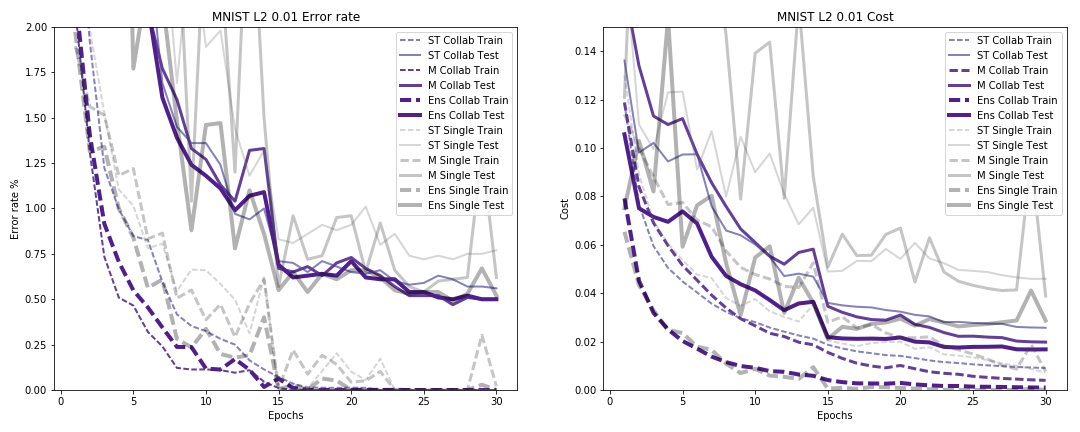
\includegraphics[scale=0.4]{{graphs/MNIST_FINAL_L2_0.01_Error}.png}\end{center}
	\caption{MNIST Collab model}\label{FinMNISTFig}
\end{figure}
\begin{figure}[H]
	\begin{center} 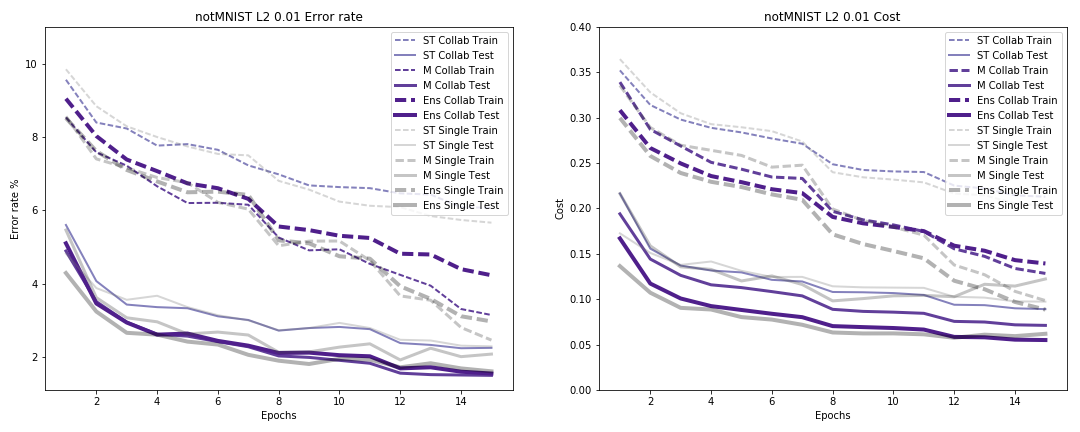
\includegraphics[scale=0.4]{{graphs/notMNIST_FINAL_L2_0.01_Error}.png}\end{center}
	\caption{notMNIST Collab model}\label{FinnotMNISTFig}
\end{figure}
\begin{figure}[H]
	\begin{center} 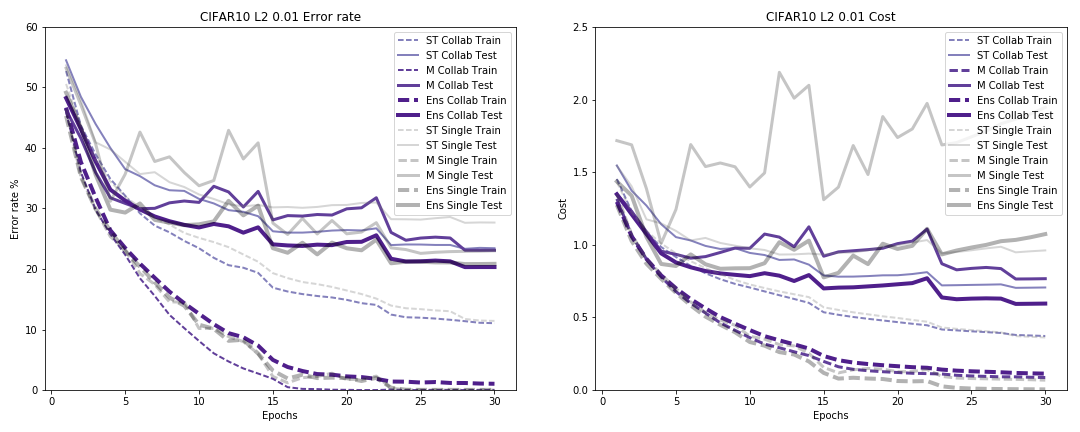
\includegraphics[scale=0.4]{{graphs/CIFAR10_FINAL_L2_0.01_Error}.png}\end{center}
	\caption{CIFAR10 Collab model}\label{FinCIFAR10Fig}
\end{figure}

\end{document}
